%% 
%% Copyright 2019-2024 Elsevier Ltd
%% 
%% This file is part of the 'CAS Bundle'.
%% --------------------------------------
%% 
%% It may be distributed under the conditions of the LaTeX Project Public
%% License, either version 1.3c of this license or (at your option) any
%% later version.  The latest version of this license is in
%%    http://www.latex-project.org/lppl.txt
%% and version 1.3c or later is part of all distributions of LaTeX
%% version 1999/12/01 or later.
%% 
%% The list of all files belonging to the 'CAS Bundle' is
%% given in the file `manifest.txt'.
%% 
%% Template article for cas-sc documentclass for 
%% double column output.

\documentclass[a4paper,fleqn]{cas-sc}

% If the frontmatter runs over more than one page
% use the longmktitle option.

%\documentclass[a4paper,fleqn,longmktitle]{cas-sc}

\usepackage[numbers]{natbib}
%\usepackage[authoryear]{natbib}
% \usepackage[authoryear,longnamesfirst]{natbib}
\usepackage{graphicx}
\usepackage{amsmath}
\usepackage{amssymb}
\usepackage{hyperref}
\usepackage{xcolor}
\usepackage{makecell}
\usepackage{caption}
\usepackage{multirow, multicol}
\usepackage{hyperref}
\usepackage{threeparttable}
\usepackage{graphicx}
\usepackage{subcaption}

%%%Author macros
\def\tsc#1{\csdef{#1}{\textsc{\lowercase{#1}}\xspace}}
\tsc{WGM}
\tsc{QE}
%%%

% Uncomment and use as if needed
%\newtheorem{theorem}{Theorem}
%\newtheorem{lemma}[theorem]{Lemma}
%\newdefinition{rmk}{Remark}
%\newproof{pf}{Proof}
%\newproof{pot}{Proof of Theorem \ref{thm}}

\begin{document}
\let\WriteBookmarks\relax
\def\floatpagepagefraction{1}
\def\textpagefraction{.001}

% Short title
\shorttitle{GuidedDCNet: A Diffusion-Integrated Framework for Enhanced Data Classification}    

% Short author
\shortauthors{M. N. Phan et~al.}  

% Main title of the paper
\title [mode = title]{GuidedDCNet: A Diffusion-Integrated Framework with Multi-Scale Conditional Guidance for Enhanced Data Classification}  

% First author
%
% Options: Use if required
% eg: \author[1,3]{Author Name}[type=editor,
%       style=chinese,
%       auid=000,
%       bioid=1,
%       prefix=Sir,
%       orcid=0000-0000-0000-0000,
%       facebook=<facebook id>,
%       twitter=<twitter id>,
%       linkedin=<linkedin id>,
%       gplus=<gplus id>]

\author[1]{Minh Nhat Phan}[orcid=0009-0008-3861-9892]
\ead{nhat0299@gmail.com}

\credit{Conceptualization, Methodology, Writing - original draft, }

\affiliation[1]{organization={The University of Danang, University of Science and Technology}, city={Da Nang}, country={Vietnam}}

\author[2]{Thi Hoang Phuong Nguyen}[orcid=0009-0009-6755-604X]
\ead{nthphuong@pdu.edu.vn}
\affiliation[2]{organization={Pham Van Dong University}, city={Quang Ngai}, country={Vietnam}}

\credit{Visualization, Writing - original draft}

\author[1]{Van Hieu Nguyen}[orcid=0000-0001-5311-806X]
\cormark[1]
\ead{nvhieuqt@dut.udn.vn}

\credit{Supervision, Writing - review and editing, Funding acquisition}
\cortext[1]{Corresponding author}

% Here goes the abstract
\begin{abstract}
Despite often achieving strong results, current classification methods tend to overuse the full features and lack flexibility due to specialized architectures. To address these challenges, this study proposes GuidedDCNet — a diffusion-integrated framework for robust classification in noisy data. Its key innovation, the Multi-scale Conditional Guidance Mechanism, enables parallel processing of global and local features, while the denoising diffusion process, implemented with conditional U-Net, is optimized via the Maximum Mean Discrepancy Loss Function to enhance generalization and stability. Comprehensive evaluations on 16 diverse datasets demonstrate that GuidedDCNet consistently outperforms existing approaches across multiple data modalities. Specifically, it achieves state-of-the-art results on one-dimensional data (99.58\% and 98.78\% on two NIR datasets), two-dimensional data (90.67\% and 96.51\% on two image datasets), and high-dimensional text data (where it surpasses ST5-XXL on 7 out of 12 datasets and significantly outperforms BERT-base, achieving an average accuracy of 71.70\% vs. 61.66\% on the MTEB benchmark), all while maintaining significantly lower parameter complexity. Furthermore, ablation studies validate the effectiveness of the proposed design, reinforcing its potential as a new paradigm for high-accuracy, multimodal classification tasks with enhanced robustness and practical applicability. Code is available at: \url{https://github.com/PhanNhat02092003/GuidedDCNet}
\end{abstract}

% Use if graphical abstract is present
\begin{graphicalabstract}
    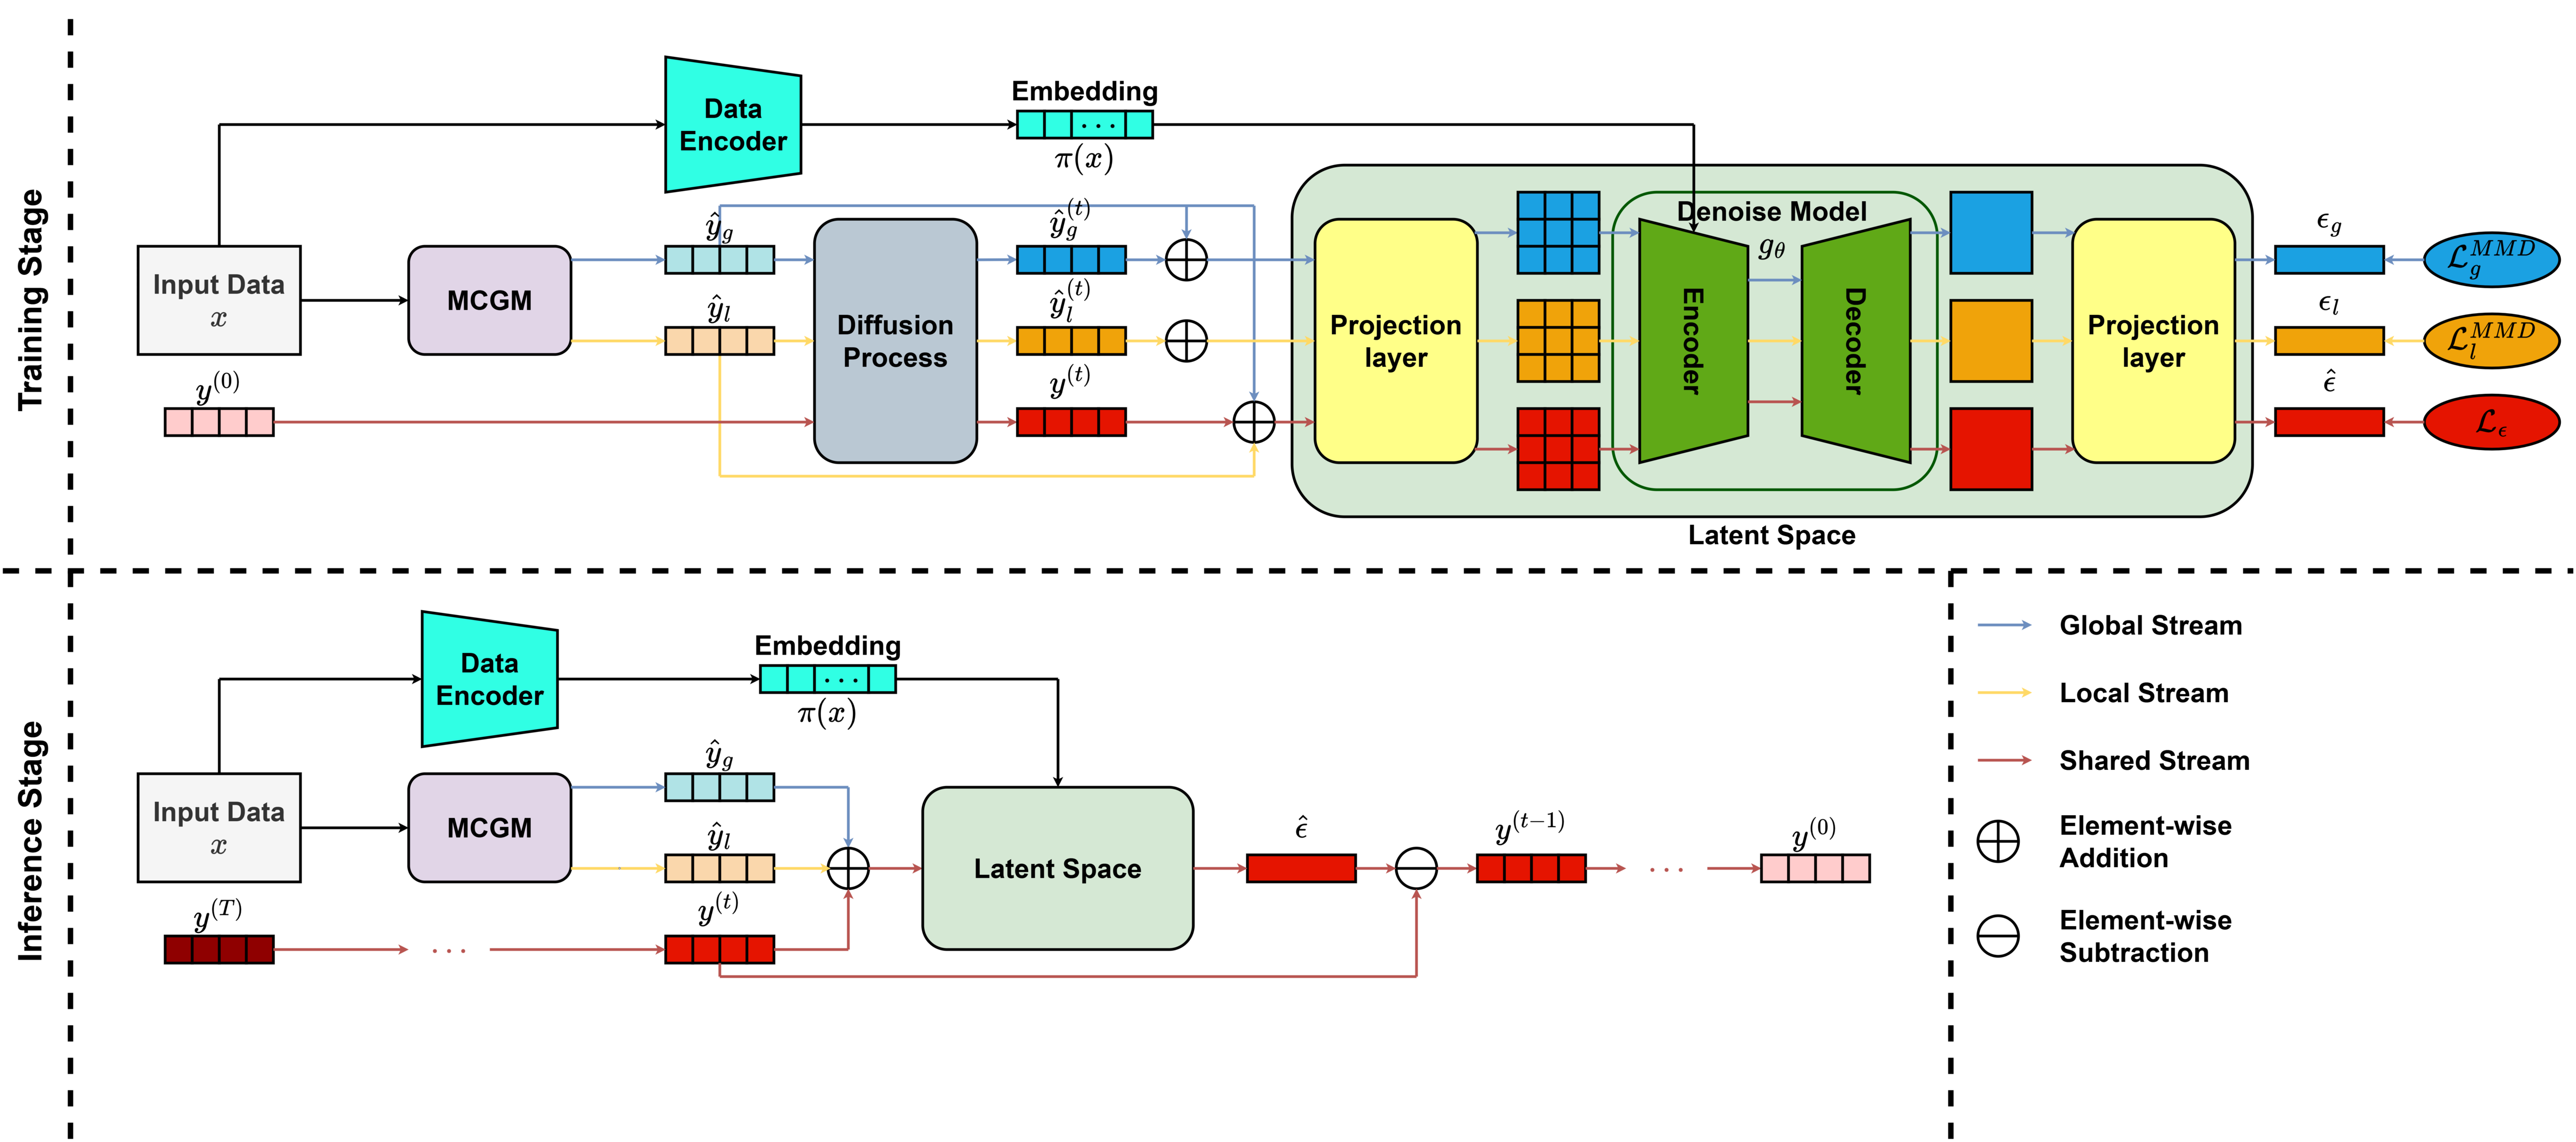
\includegraphics[width=\linewidth]{figs/Fig1.png}
\end{graphicalabstract}

% Research highlights
\begin{highlights}
    \item Proposal of a Novel Diffusion-integrated Classification Framework GuidedDCNet
    \item Introduction of the Multi-scale Conditional Guidance Mechanism
    \item Comprehensive Evaluation Across Multiple Classification Tasks
\end{highlights}


% Keywords
% Each keyword is seperated by \sep
\begin{keywords}
    GuidedDCNet \sep diffusion-based classification \sep Multi-scale Conditional Guidance \sep noisy data robustness \sep Maximum Mean Discrepancy Loss
\end{keywords}

\maketitle

% Main text
\section{Introduction}
Data classification remains a fundamental challenge in machine learning, playing a crucial role across diverse domains from signal processing and computer vision to natural language processing  \cite{sarker2021deep,akinci2024machine,joshi2022deep,zhang2022review}. The evolution of classification models has seen remarkable progress, from traditional machine learning approaches like Support Vector Machines (SVM) \cite{cortes1995support}, Random Forests \cite{breiman2001random}, through early neural networks like Multi-Layer Perceptrons (MLPs) \cite{kruse2022multi} to increasingly sophisticated architectures. Convolutional Neural Networks (CNNs) have evolved from AlexNet through VGGNet, ResNet, and DenseNet to modern variants like EfficientNet and ConvNeXt \cite{jo2023convolutional}. Sequential data modeling has progressed from basic Recurrent Neural Networks (RNNs) to advanced architectures like LSTM, GRU \cite{jo2023recurrent}. More recently, Transformer-based models \cite{vaswani2017attention} have revolutionized the field, spawning variants like Vision Transformer (ViT) \cite{dosovitskiy2021an}, Swin Transformer \cite{liu2021swin} for vision tasks, while BERT \cite{devlin2019bert} has dominated natural language processing. Each advancement has brought significant improvements in classification accuracy and capability across different data modalities.

However, despite these advances, current classification approaches face three fundamental challenges. First, the holistic processing nature of traditional single-encoder models leads to both redundant information capture and failure to focus on key discriminative features, especially problematic when dealing with noisy real-world data. Second, while recent studies on multi-scale feature extraction \cite{luo2021apple,dai2025mtmfnet,zhu2024diffusion,gao2025msfm} have shown promise, balancing the contributions of global and local features remains challenging due to their different scales and semantic levels. Third, existing architectures are often specialized for specific data types and rely heavily on increased model complexity for performance gains, an approach that shows diminishing returns in real-world applications \cite{sarker2021deep,akinci2024machine}. These limitations highlight the need for a unified, noise-robust approach to classification that can maintain effectiveness across different data modalities without excessive architectural scaling.

Building upon these advantages, this study introduces GuidedDCNet, a novel Denoising Diffusion-based model designed to improve accuracy in data classification. Developed upon the principles of advanced probabilistic diffusion models, the proposed approach effectively mitigates unwanted noise in input data by leveraging the stochastic nature of the diffusion process at each sampling step. To enhance the denoising capability, this work proposes the Multi-scale Conditional Guidance Mechanism (MSCGM), which integrates both global and local guidance vectors throughout the diffusion process. This mechanism enables the model to analyze data across multiple levels. Notably, by applying the diffusion process to smaller data patches, the method facilitates the precise identification of critical features within the dataset. Furthermore, the performance of GuidedDCNet is systematically evaluated across three distinct classification tasks: Near-infrared Spectroscopy classification, image classification, and text classification. The empirical findings highlight that the proposed diffusion-integrated classification framework enhances the performance of existing models, demonstrating the potential of diffusion-based approaches to advance data classification techniques.
The key contributions of this work are highlighted as follows:
\begin{enumerate}
    \item Proposal of a Novel Diffusion-integrated Classification Framework - GuidedDCNet
    \item Introduction of the Multi-scale Conditional Guidance Mechanism
    \item Comprehensive Evaluation Across Multiple Classification Tasks
\end{enumerate}
The structure of this paper is summarized as follows:
\begin{itemize}
    \item \textbf{Section 2} reviews the related works and discusses the research gap motivating our approach.
    \item \textbf{Section 3} presents the proposed method in detail, including the system architecture and algorithmic design.
    \item \textbf{Section 4} describes the experimental setup, datasets, reports, and analyzes the experimental results, comparing our method with existing approaches.
    \item \textbf{Section 5} concludes the paper and outlines potential directions for future work.
\end{itemize}


\section{Related Work}
\subsection{Applications of Denoising Diffusion Probalistic Models}

Denoising Diffusion Probabilistic Models (DDPMs) have emerged as a groundbreaking approach in generative modeling, demonstrating remarkable versatility across numerous computer vision applications \cite{croitoru2023diffusion}. The foundational work by \cite{ho2020denoising}, through the novel connection between diffusion models, denoising score matching, and Langevin dynamics, DDPMs achieved results comparable to ProgressiveGAN on 256x256 resolution images while demonstrating strong performance on the CIFAR10 dataset. This success laid the groundwork for applying DDPMs across diverse domains.

Building upon this foundation, DDPMs have shown exceptional capabilities in basic generative tasks. In image generation and manipulation, models like Imagen \cite{saharia2022photorealistic} and Stable Diffusion \cite{rombach2022high} demonstrated unprecedented abilities in text-to-image synthesis through effective embedding conditioning. The framework's success in image tasks naturally extended to video applications \cite{ho2022video,yang2023diffusion,hoppe2022diffusion}, where models effectively capture temporal dependencies for generation and prediction tasks. These successes have led to numerous domain-specific applications, particularly in medical imaging, where DDPMs have made substantial contributions. For instance, in 3D medical image generation, \cite{khader2023denoising} demonstrated effectiveness through novel latent-space diffusion architectures for MRI and CT scans. 

Beyond generative tasks, DDPMs have demonstrated significant potential in discriminative applications, particularly in classification tasks. Notably, the pioneering work of D2C \cite{de2022d2c} introduced diffusion models for few-shot conditional generation and classification. Building upon this foundation, SpectralDiff \cite{chen2023spectraldiff} further advanced the application to hyperspectral image classification, achieving notably improved accuracy. In the medical domain, this trend continued with DiffMIC-v2 \cite{yang2025diffmic}, which pioneered diffusion-based classification for medical imaging. Not only did it achieve superior performance across diverse modalities, but it also maintained 3× better computational efficiency. Moreover, the denoising diffusion autoencoder (DDAE) \cite{xiang2023denoising} marked a significant breakthrough by unifying both generative and discriminative capabilities, attained 95.9\% accuracy on CIFAR10 and 50.0\% on Tiny-ImageNet—all without requiring auxiliary encoders.

Notably, diffusion models have exhibited strong performance in semantic segmentation \cite{luo2025label,wu2024medsegdiff}, reinforcing their broad applicability in discriminative modeling. Beyond visual tasks, their versatility extends to discrete and categorical data, particularly in natural language processing applications \cite{hoogeboom2021argmax,austin2021structured}, highlighting their potential for broader adoption beyond computer vision. In parallel, research has increasingly focused on developing multi-task and general-purpose diffusion frameworks \cite{blattmann2022retrieval,graikos2022diffusion,gao2021learning}, demonstrating how a single model can integrate various generative and manipulative processes within a unified architecture.

This evolution from basic image generation to advanced multi-purpose frameworks highlights DDPMs as a foundational approach for developing unified architectures capable of handling diverse data modalities. 

\subsection{Existing Classification Approaches}

Data classification has evolved through several significant milestones, from traditional machine learning approaches to modern deep learning architectures.

Traditional classification methods, such as Support Vector Machines (SVM) \cite{cortes1995support} and Random Forests \cite{breiman2001random}, have long served as the foundation of pattern recognition. Kernel methods \cite{scholkopf2002learning} expanded the capability to handle non-linear data, while ensemble learning \cite{dietterich2000ensemble} enhanced robustness by combining multiple base models. Subsequently, boosting-based algorithms such as AdaBoost \cite{ying2013advance}, XGBoost \cite{niazkar2024applications}, and LightGBM \cite{ke2017lightgbm} significantly improved computational efficiency and accuracy through gradient optimization and parallel learning. These approaches achieved strong results on tabular and structured datasets, but their reliance on handcrafted features and limited scalability often restricted their performance on complex, high-dimensional, or unstructured data such as images or text.

The foundations of deep learning in image classification were established with LeNet \cite{lecun2002gradient}, which pioneered Convolutional Neural Networks (CNNs) for handwritten digit recognition. A transformative breakthrough came with AlexNet \cite{krizhevsky2012imagenet}, which demonstrated the unprecedented potential of deep CNNs by winning the ImageNet Challenge, marking the beginning of the deep learning era. Following this success, architectures such as VGGNet \cite{donelly2012very}, ResNet \cite{he2016deep}, and DenseNet \cite{huang2017densely} improved gradient flow and feature reuse through skip and dense connections, significantly deepening network capacity. Further advancements such as EfficientNet \cite{tan2019efficientnet} and EfficientNetV2 \cite{tan2021efficientnetv2} introduced compound scaling and progressive learning, achieving a balance between accuracy and computational cost.

Although CNNs have proven effective in learning hierarchical features, they remain limited in modeling long-range dependencies. To address this limitation, the introduction of the Transformer architecture \cite{vaswani2017attention} introduced self-attention mechanisms that enable global context modeling. Vision Transformer (ViT) \cite{dosovitskiy2021an} successfully extended this architecture to image classification, while Swin Transformer \cite{liu2021swin} and DiNAT \cite{hussein2023dilated} enhanced scalability and efficiency through hierarchical and dilated attention mechanisms. In addition, hybrid architectures such as CoAtNet \cite{dai2021coatnet}, ConvNeXt \cite{liu2022convnet}, and ConvNeXtv2 \cite{woo2023convnext} have attempted to bridge convolutional inductive biases with attention-based global modeling, achieving state-of-the-art performance across diverse classification tasks.

Parallel to the development of attention models, another promising research direction emerged through diffusion models \cite{ho2020denoising,dhariwal2021diffusion,chen2023spectraldiff,yang2025diffmic,de2022d2c}, attracting particular attention for their ability to model complex data distributions. In this field, Dhariwal and Nichol \cite{dhariwal2021diffusion} achieved a significant breakthrough by integrating U-Net architecture and attention into diffusion models. More notably, the application of diffusion models in classification tasks through D2C \cite{de2022d2c} and advanced models such as SpectralDiff \cite{chen2023spectraldiff} and DiffMIC-v2 \cite{yang2025diffmic} has opened new prospects in learning discriminative features. 

Recent studies have extended this line of work by formalizing diffusion-based discriminative modeling. For instance, Classification Diffusion Models \cite{yadin2024classification} reformulate diffusion inference through density-ratio estimation, providing a principled connection between diffusion dynamics and discriminative decision boundaries. Likewise, Diffusion Models are Certifiably Robust Classifiers \cite{chen2024diffusion} demonstrated that diffusion-based classifiers can offer theoretical robustness guarantees, highlighting their potential advantages over conventional discriminative networks. In parallel, hybrid and task-specific diffusion frameworks such as SpectralDiff \cite{chen2023spectraldiff}, DiffCRN \cite{zhu2025spatial}, and DiffCR \cite{zou2024diffcr} leverage spectral cues and contrastive regularization to enhance discriminative feature learning in challenging domains such as hyperspectral and medical imaging. Together, these approaches underline the growing interest in bridging generative diffusion modeling with discriminative representation learning.

However, diffusion models' application to classification tasks still faces several limitations. First, the potential of the diffusion process’s denoising capabilities for improving classification robustness remains largely unexplored. Second, existing methods such as SpectralDiff and DiffMIC-v2 \cite{chen2023spectraldiff,yang2025diffmic} lack effective mechanisms for multi-scale feature analysis, particularly in combining global and local information. Additionally, the challenge of maintaining consistent performance across different data types without major architectural changes persists \cite{ho2020denoising}. These limitations motivate our proposed GuidedDCNet, which leverages the stochastic diffusion process with multi-scale conditional guidance to enhance classification performance across various data types.

The proposed GuidedDCNet distinguishes itself by introducing a Multi-scale Conditional Guidance Mechanism (MCGM) that integrates conditional information directly into the diffusion stages, rather than applying a single deterministic condition after encoding as in prior methods. Specifically, MCGM jointly injects global and local guidance vectors into the stochastic denoising trajectory, enabling explicit interaction between semantic-level and structure-level representations at each diffusion step. This integration effectively combines the strengths of diffusion modeling (progressive denoising and uncertainty handling) with multi-scale feature learning (contextual and spatial awareness) to enhance classification robustness.

In addition, guidance-specific MMD and MSE optimization are applied to the predicted noise components of global, local, and dual guidance branches, ensuring consistent and stable feature refinement across scales. Unlike previous works that treat multi-scale or diffusion concepts independently, GuidedDCNet unifies them within a single probabilistic training framework tailored for classification. Furthermore, the network is implemented as a modular plug-in, seamlessly attachable to existing encoder architectures to strengthen representation learning and maintain high generalization across diverse data modalities—without requiring architectural redesign.

\section{Proposed Method}
Figure \ref{fig1} illustrates an overview of the proposed network architecture, GuidedDCNet, designed for classification. Given an input sample \( x \), the data undergoes initial processing through an encoder, which extracts a feature embedding denoted as \( \pi(x) \). Concurrently, a Multi-scale Conditional Guidance Mechanism (MCGM) generates both a global guidance vector \( \hat{y}_g \) and a local guidance vector \( \hat{y}_l \). During the training phase, a diffusion process is applied to the ground truth label \( y_0 \), incorporating the guidance vectors to yield three distinct noisy variables: \( y_g^{(t)} \) (global guidance), \( y_l^{(t)} \) (local guidance), and \( y^{(t)} \) (dual guidance). These noisy representations, along with their corresponding guidance vectors, are subsequently projected into a latent space. The projected embeddings are then integrated with the feature embedding \( \pi(x) \) and processed through a denoising U-Net to estimate the noise distributions associated with \( y_g^{(t)} \), \( y_l^{(t)} \), and \( y^{(t)} \). Furthermore, a maximum mean discrepancy (MMD) regularization adapted to specific guidances is introduced for the estimated noise associated with \( y_g^{(t)} \) and \( y_l^{(t)} \) to enhance the robustness of noise prediction. Simultaneously, a noise estimation loss based on the mean squared error (MSE) criterion is employed for the predicted noise of \( y^{(t)} \). This comprehensive training strategy facilitates the collaborative optimization of the GuidedDCNet network, thereby improving its classification performance. GuidedDCNet is designed as a flexible framework rather than a large-scale standalone classifier. Its primary goal is to improve the representation and classification quality of existing base models when integrated into their data encoder modules. 

\begin{figure}[!ht]
    \centering
    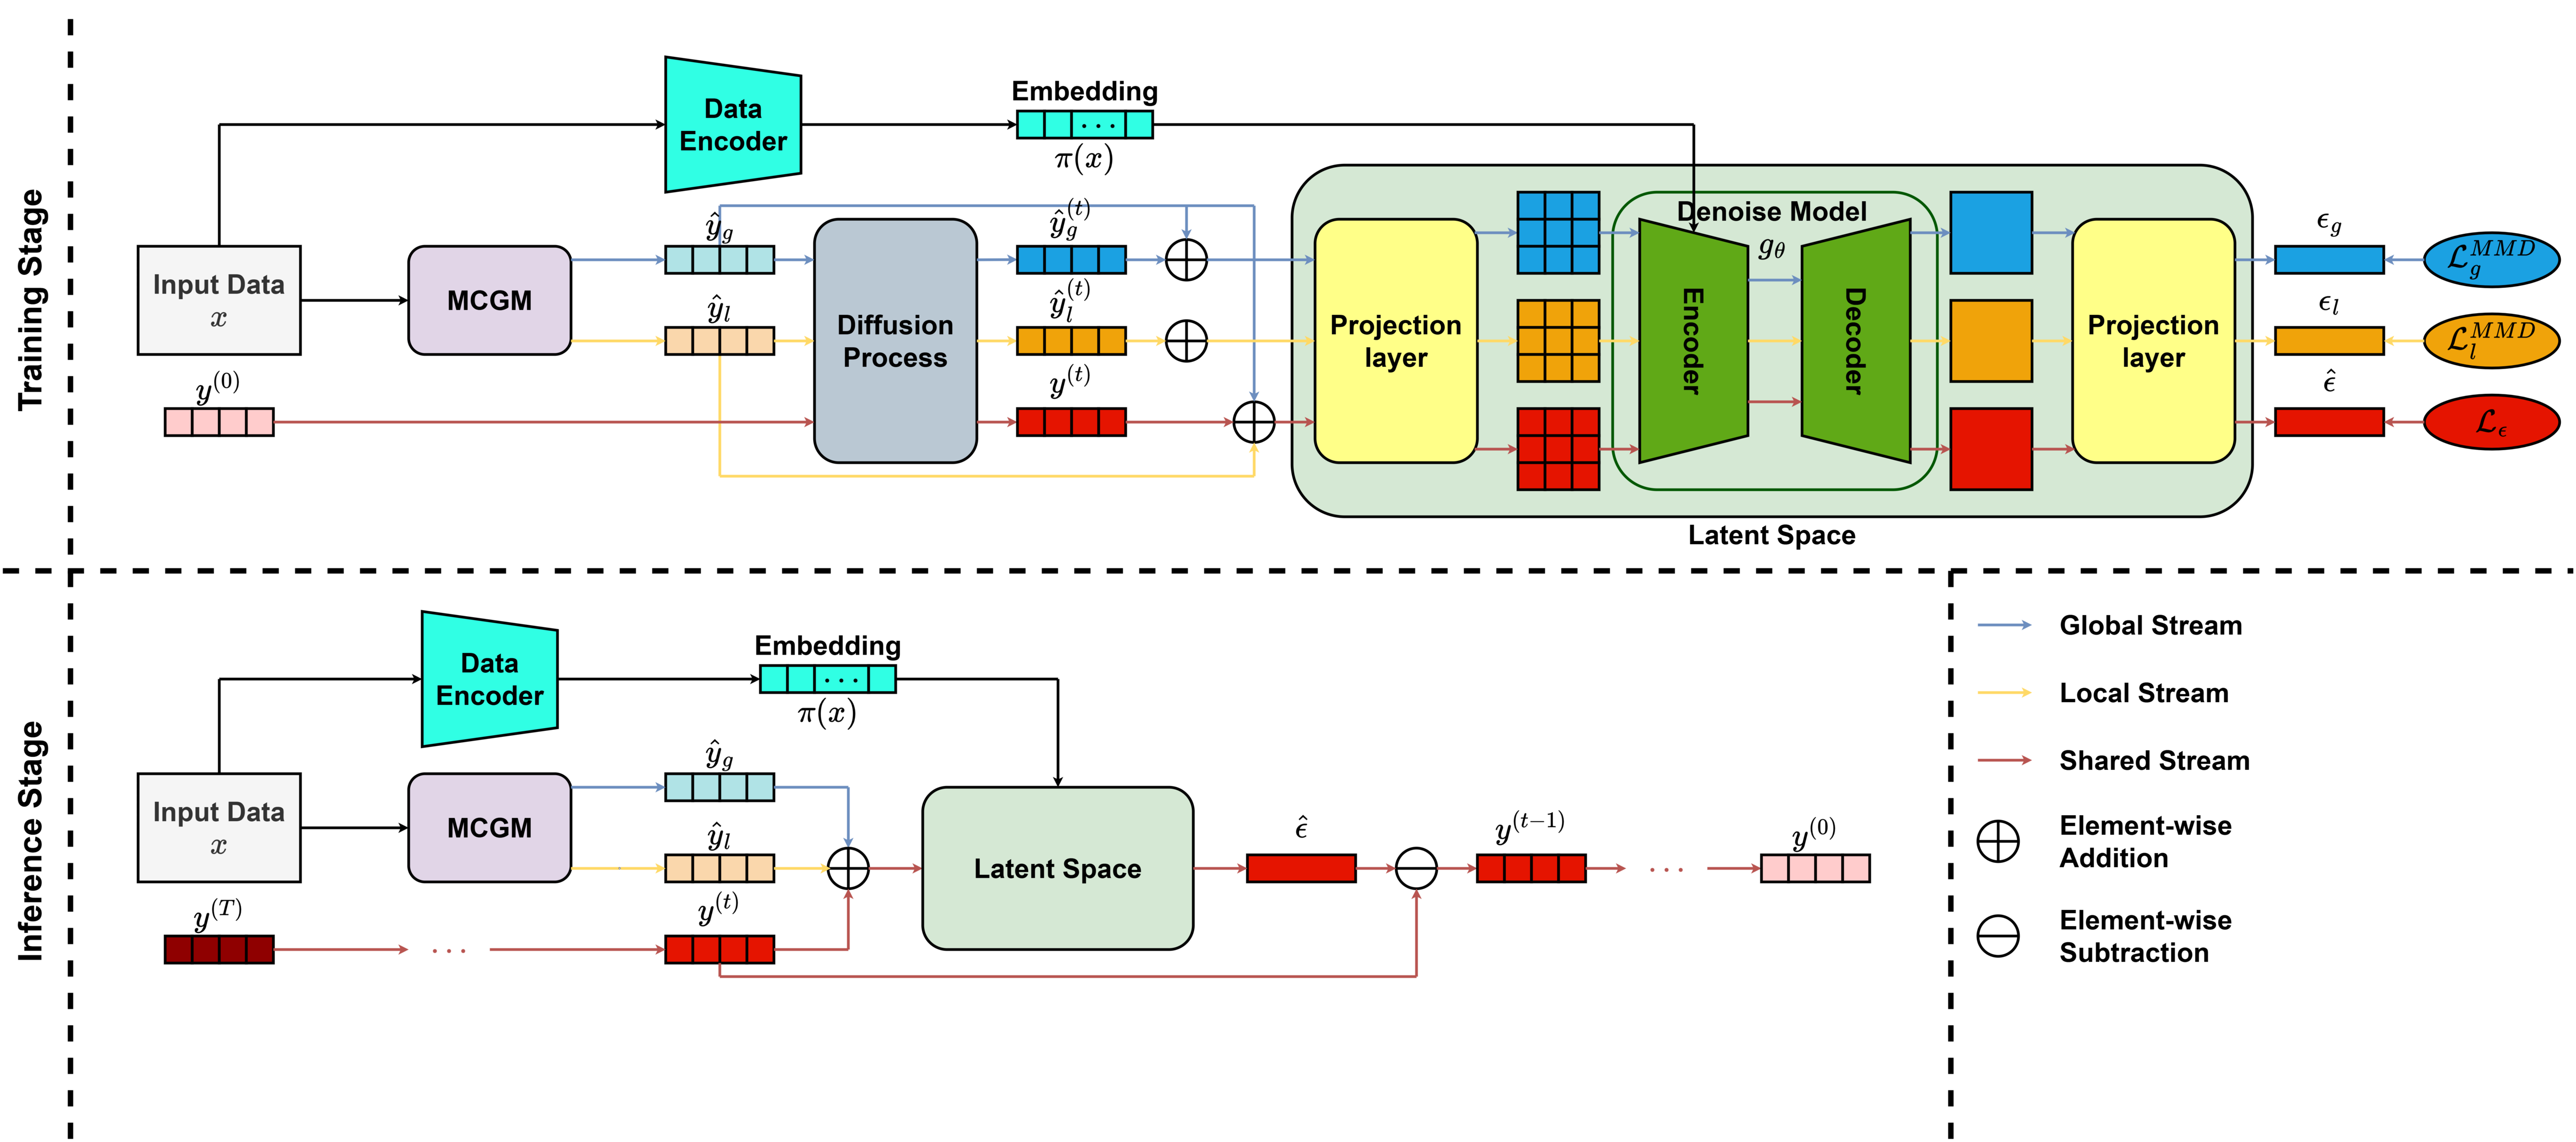
\includegraphics[width=\linewidth]{figs/Fig1.png}
    \caption{GuidedDCNet Overall Architecture}
    \label{fig1}
\end{figure}

\subsection{Multi-scale Conditional Guidance Mechanism}
In conditional Denoising Diffusion Probabilistic Models (DDPMs), data classification remains a significant challenge due to the inherent ambiguity associated with object representations within the dataset. The process of accurately identifying and distinguishing various attributes within the data is often complex, as objects may exhibit overlapping characteristics that hinder precise differentiation. This issue is further exacerbated by the presence of noise and artifacts within the most influential regions within the data, which can obstruct the extraction of meaningful high-level semantic features. Such noise may arise from multiple sources, including sensor inaccuracies, environmental variations, and intrinsic data inconsistencies, all of which contribute to the difficulty of learning discriminative representations necessary for robust classification.  

A fundamental limitation of many existing DDPM-based classification approaches is their reliance on raw initial data as the sole conditioning factor in each diffusion step. While this data provides a foundational input for the learning process, it is often insufficient for capturing the fine-grained, high-resolution details required for effective classification. The absence of additional contextual information and feature refinement mechanisms impairs the model’s ability to discern subtle variations, particularly among visually or semantically similar categories. Consequently, this constraint leads to suboptimal classification performance, as the model is unable to fully exploit the available data to generate precise predictions. To address these challenges, it is imperative to develop enhanced conditioning strategies that incorporate richer contextual features, mitigate the influence of noise, and facilitate the extraction of more discriminative representations throughout the diffusion process.

To address the aforementioned challenge, a Multi-scale Conditional Guidance Mechanism (MCGM) is proposed to refine the encoding process at each step of the diffusion process. Specifically, the MCGM model \( f_{MCGM} \) is introduced to compute guidance vectors at both global and local levels, thereby facilitating more effective information propagation and improving the robustness of the diffusion framework.

\begin{figure}[!ht]
    \centering
    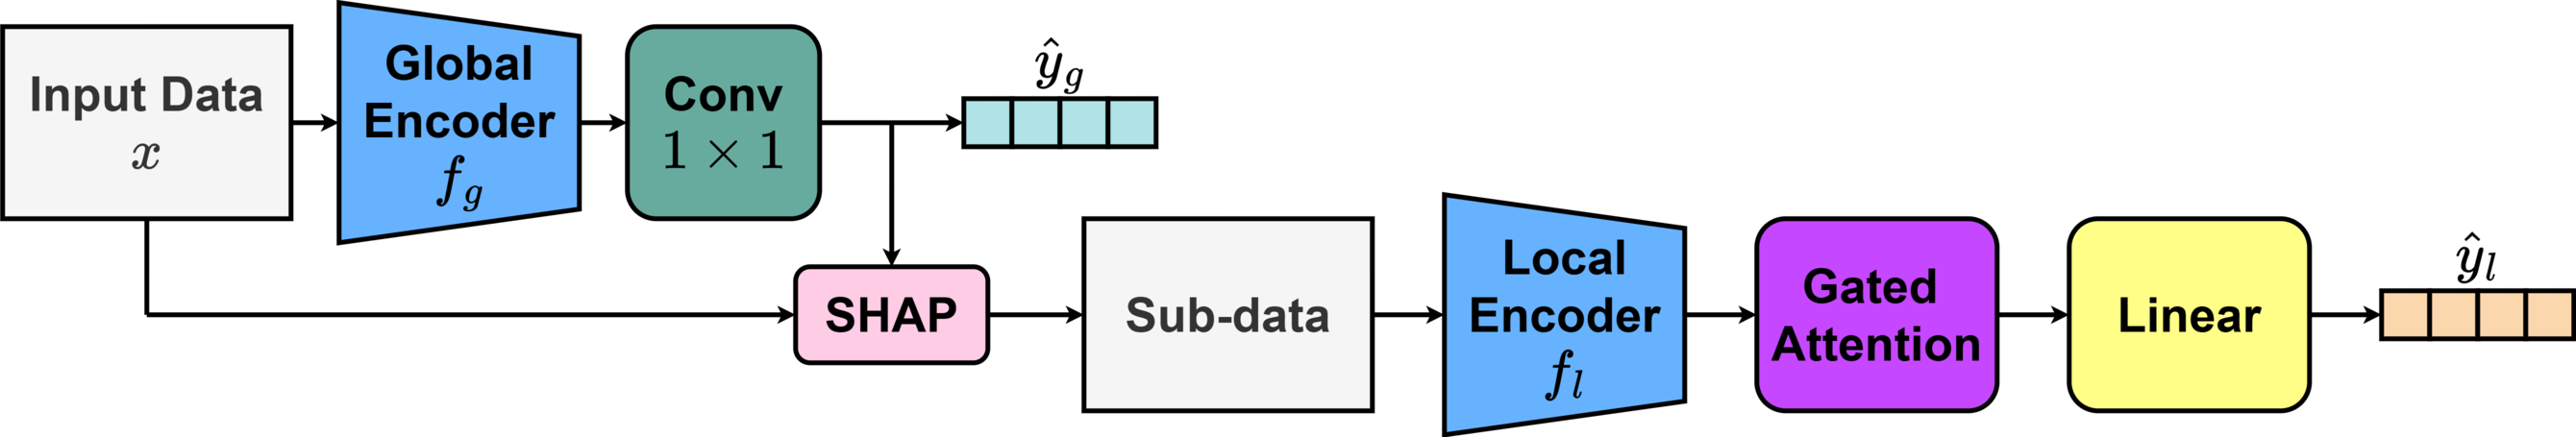
\includegraphics[width=\linewidth]{figs/Fig2.png}
    \caption{Multi-scale Conditional Guidance Mechanism}
    \label{fig2}
\end{figure}

A holistic representation of the data distribution is provided by the global guidance vector, enabling a comprehensive contextual understanding. In contrast, the local guidance vector allows selective focus on the most influential regions within the data, where critical information is contained for mitigating the impact of noise. As depicted in Figure \ref{fig2}, this mechanism is implemented through a dual-stream architecture.  

To begin with, the input data \( x \) is embedded by the global encoder \( f_g \), followed by a \( 1 \times 1 \) convolutional layer, through which an attention map representing the overall distribution of prominent features is generated. The global guidance vector \( \hat{y}_g \) is subsequently obtained by computing the average response across this saliency map, ensuring a stable global guidance vector for diffusion.  

In the local stream, Shapley Additive Explanations (SHAP) \cite{lundberg2017unified} is employed to identify and extract the most influential regions within the data by quantifying the contribution of individual features to the model’s predictions. Based on these identified key features, a refined subset of the data is subsequently constructed to facilitate further analysis. The sub-data is then processed by the local encoder \( f_l \), and distinct feature representations are generated. To effectively aggregate these features, a gated attention mechanism \cite{rodriguez2018attend} is employed, which adaptively assigns importance weights to different sub-data features. The resulting weighted feature representation is then passed through a linear layer, where the local guidance vector \( \hat{y}_l \) is computed, thereby enhancing the model’s capacity to capture fine-grained details while effectively suppressing noise.

The outputs of the Multi-scale Conditional Guidance Mechanism, namely the global guidance vector $y_g$ and the local guidance vector $y_l$, are subsequently integrated and refined through the Conditional UNet within the diffusion framework, as illustrated in Figure \ref{fig3}. Specifically, these guidance vectors serve as conditioning inputs to the diffusion model, enabling the network to adaptively modulate the denoising process according to both global contextual information and localized salient features. Through this integration, the Conditional UNet fuses multi-scale semantic cues derived from Figure \ref{fig2} with the timestep and noisy representations at each diffusion step, thereby enhancing semantic consistency and improving the accuracy of noise estimation across different data scales.

\subsection{Diffusion Model}
Our proposed diffusion model adopts a two-stage framework analogous to Denoising Diffusion Probabilistic Models (DDPM) \cite{ho2020denoising}, consisting of a diffusion process and a denoising process.

During the forward diffusion stage, the target variable \( y^{(0)} \) is incrementally perturbed by the addition of Gaussian noise at each time step. These time steps are sampled from a uniform distribution over the interval \([1,T]\), generating a sequence of progressively noised variables denoted as \(\{y^{(1)},\ldots, y^{(t)},\) \(\ldots y^{(T)}\} \). This process serves to construct a latent representation that facilitates effective noise modeling.  

Following the training phase, the reverse diffusion process is executed to recover the original response variable. To parameterize this process, we use a conditional UNet architecture as the denoising network, following the standard DDPM implementation, as illustrated in Figure \ref{fig3}. The trained UNet \( g_\theta \) with the set of trainable parameters \( \theta \) is tasked with generating the final prediction \( \hat{y}^{(0)} \) by transforming the distribution of the noisy variable \( p_\theta(y^{(T)}) \) back to the original data distribution \( p_\theta(y^{(0)}) \).  

\begin{figure}
    \centering
    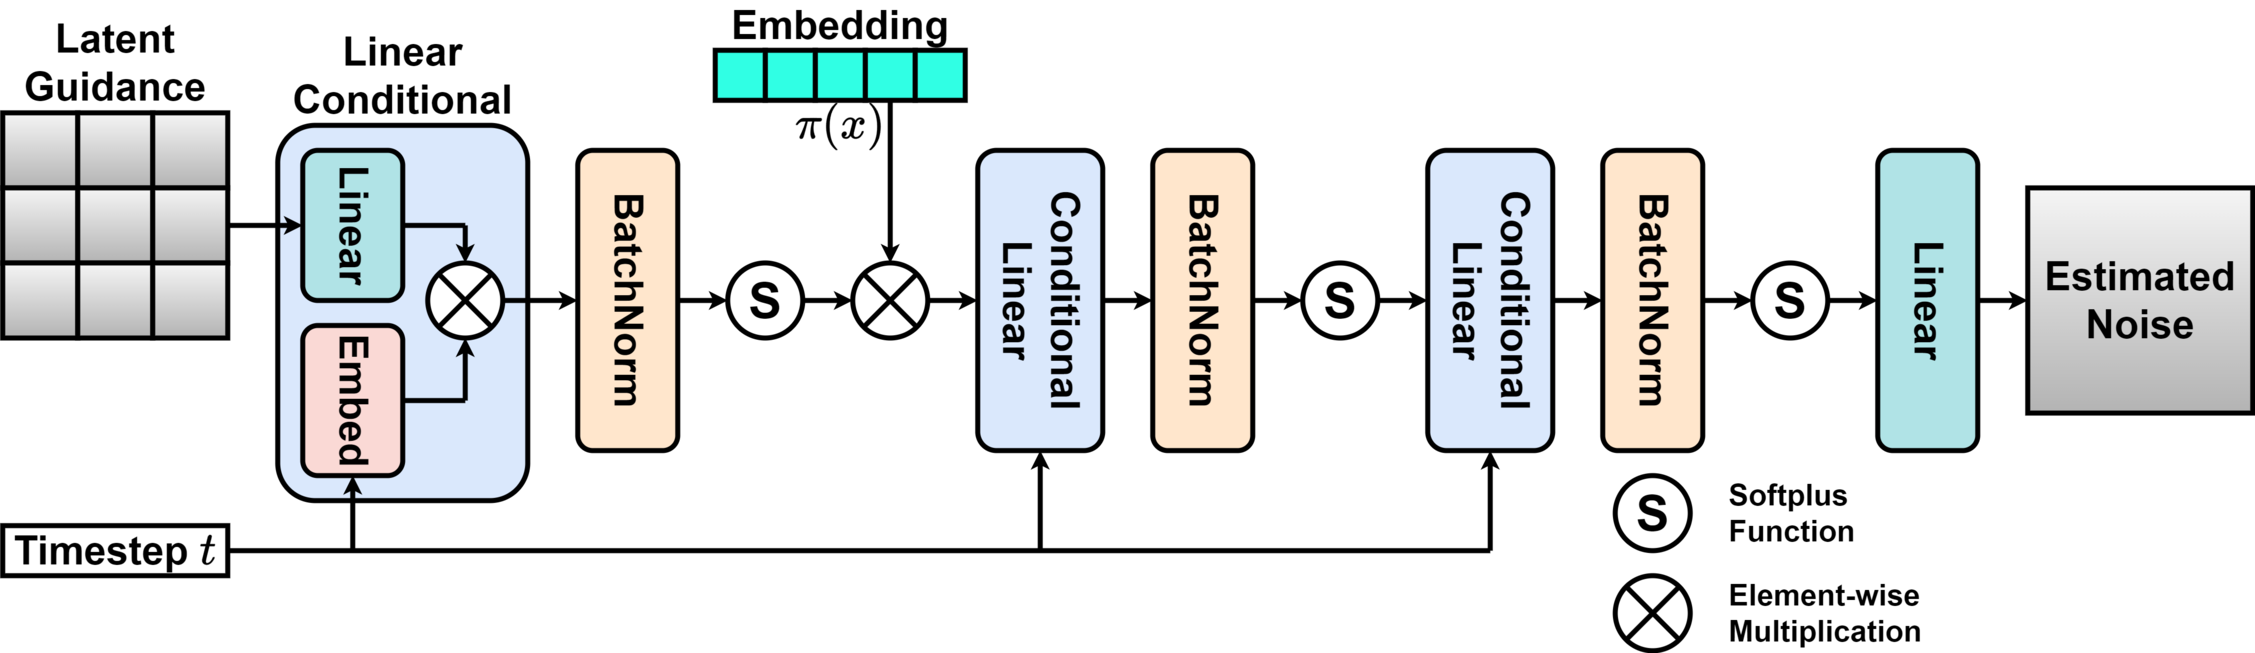
\includegraphics[width=\linewidth]{figs/Fig3.png}
    \caption{Conditional UNet Architecture}
    \label{fig3}
\end{figure}

With the initialization of the noisy variable follows the Gaussian distribution \(p_\theta(y^{(T)}) = \mathcal{N}\left(\frac{\hat{y}_g + \hat{y}_l}{2}, I\right)\), the reverse diffusion process is formulated as:  
\begin{equation}
    p_\theta(y^{(0:T-1)} | y^{(T)}, \pi(x)) = \prod_{t=1}^{T} p_\theta(y^{(t-1)} | y^{(t)}, \pi(x))    
\end{equation}

This process defines the probabilistic generative process in which the model iteratively estimates the cleaner latent variable $y^{(t-1)}$ from its noisier version $y^{(t)}$. To establish the correspondence between this reverse process and its forward diffusion counterpart, we explicitly define how each noisy variable $y^{(t)}$ is constructed during the forward process. This connection ensures that the reverse model operates on well-defined noise-corrupted samples governed by a consistent diffusion schedule. Accordingly, the noisy variable at each timestep $t$ is obtained as follows:  
\begin{equation}
    y^{(t)} = \sqrt{\bar{\alpha_t}} y^{(0)} + \sqrt{1 - \bar{\alpha_t}} \epsilon + (1 - \sqrt{\bar{\alpha_t}})(\hat{y_g} + \hat{y_l}),
\end{equation}
where \( \epsilon \sim N(0, I) \), \( \bar{\alpha_t} = \prod_t\alpha_t \), and \( \alpha_t = 1 - \beta_t \) with a linear noise schedule \(\{ \beta_t|\beta_t \in (0,1) \}_{t=1:T}\).  

Following the sampling process, the noisy variable \( y^{(t)} \) is further refined through the incorporation of dual guidance vectors \( (\hat{y_g}, \hat{y_l}) \) before being input into the denoising model UNet \( g_{\theta} \). The primary objective of UNet is to estimate the noise distribution, which is formally expressed as:  
\begin{equation}
    g_{\theta}(\pi(x), y^{(t)}, \hat{y_g}, \hat{y_l}, t) = \text{Dec}\left(\text{Enc}\left(\text{Proj}\left(\text{Concat}\left(y^{(t)}, \hat{y_g}, \hat{y_l}\right)\right), \pi\left(x\right), t\right), t\right),
\end{equation}
where \( Proj(\cdot) \) denotes the projection layer mapping data to the latent space, \( Enc(\cdot) \) and \( Dec(\cdot) \) correspond to the encoder and decoder components of the UNet architecture, respectively.  

Figure \ref{fig3} illustrates the proposed Conditional UNet Architecture, which augments the conventional diffusion process through explicit timestep conditioning and semantic feature guidance. This design enables the model to exploit both temporal and contextual information during the denoising procedure, thereby improving representational fidelity and semantic consistency. Let $y^{(t)}$ denote the noisy observation at the diffusion step $t$. The corresponding timestep is first embedded into a continuous representation by a learnable embedding function:
\begin{equation}
    e^t=\text{Embed}(t)
\end{equation}
The noisy input is projected into the latent space through a linear transformation, and temporal conditioning is applied via element-wise interaction between the two representations:
\begin{equation}
    z_1=\left(W_1y^{(t)}\right)\odot e_t
\end{equation}
where $W_1$ is a learnable weight matrix and $\odot$ represents the Hadamard product. This operation allows the network to internalize temporal dynamics directly within its latent representation. To further enhance semantic awareness, the data feature embedding $\pi(x)$, extracted from the original input $x$, is subsequently integrated with the temporally conditioned vector:
\begin{equation}
    z_2 = z_1\odot \pi(x)
\end{equation}
This semantic modulation step ensures that the network remains guided by high-level contextual cues derived from the input distribution, enabling more meaningful and structurally coherent denoising.

The resulting feature vector $z_2$ is then processed through a hierarchy of Conditional Linear Blocks, each comprising a linear transformation, Batch Normalization, and a Softplus activation. At each block, the timestep embedding is reintroduced through element-wise modulation to preserve temporal consistency:
\begin{equation}
    z_{k+1}=\text{Softplus}\left(\text{BatchNorm}\left(W_k z_k\odot e_t\right)\right),\quad k=2,3,\ldots,K.
\end{equation}
This recurrent incorporation of $e_t$ across network depths enforces temporal coherence and improves gradient stability throughout the training process. Finally, the network produces an estimated noise component through a terminal linear projection:
\begin{equation}
    \epsilon^{(t)}=W_{out}z_K
\end{equation}
where $W_{out}$ maps the latent representation back to the data dimensionality. For stability, all linear layers (except the output layer) are followed by Batch Normalization and Softplus activation, promoting smooth gradient propagation and mitigating vanishing or exploding gradient issues.

In summary, the proposed architecture can be formulated as a conditional mapping:
\begin{equation}
    \epsilon^{(t)}=f_\theta\left(y^{(t)},e_t,\pi\left(x\right)\right)
\end{equation}
where $f_\theta(\cot)$ denotes the Conditional UNet parameterized by $\theta$. By conditioning each denoising step on both the timestep and semantic embeddings, the network effectively aligns temporal dynamics with contextually salient regions of the data, resulting in enhanced noise estimation accuracy, improved robustness, and more semantically consistent generative performance.

\subsection{Loss Function}
Maximum-Mean Discrepancy (MMD) quantifies the difference between two distributions by analyzing discrepancies in their statistical properties \cite{keller2025histokernel,sun2024mmd}, efficiently computed using a positive definite kernel \( \mathbb{K}(\cdot,\cdot) \) that reproduces distributions in Hilbert space. Inspired by these studies \cite{zhao2019infovae,sinha2021d2c,huang2018introvae}, a combination of MMD regularization functions is introduced to enhance the learning of mutual information between the noise-generating distribution and the reference normal distribution.  

In our approach, the noisy variable \( y_g^{(t)} \) is sampled from the diffusion stage at timestep \( t \), informed by the global guidance vector. The MMD loss is defined as:  
\begin{equation}\label{eq1}
    \mathcal{L}^{MMD}_{g}(\epsilon||m) = \mathbb{K}(\epsilon,\epsilon')-2\mathbb{K}(\epsilon_g,\epsilon)+\mathbb{K}(\epsilon_g,\epsilon_g'),    
\end{equation}
where \(\epsilon_g = g_{\theta}\left(\pi\left(x\right),\ \sqrt{\bar{\alpha_t}} y^{(0)} + \sqrt{1 - \bar{\alpha_t}} \epsilon + \left(1 - \sqrt{\bar{\alpha_t}}\right) \hat{y_g},\ \hat{y_g},\ t\right)\). This MMD regularization in Equation \ref{eq1} is also employed for the local guidance vector to compute \( \mathcal{L}^{MMD}_{l} \), as illustrated in Figure \ref{fig1}. 

During the diffusion process, model optimization is performed by minimizing the noise estimation loss \( \mathcal{L}_{\epsilon} \), defined as follows:  
\begin{equation}
    \mathcal{L}_{\epsilon} = {||\epsilon - g_{\theta}(\pi(x), y^{(t)}, \hat{y_g}, \hat{y_l}, t)||}^2.    
\end{equation}

Leveraging the generalized noise prediction capability of the loss function \( \mathcal{L}_{\epsilon} \) and the MMD regularizer effectively improves feature learning, accelerates model convergence, and enhances stability. The total loss function \( \mathcal{L}_{total} \) for GuidedDCNet is formulated by integrating the noise estimation loss with the MMD regularization terms, expressed as follows:  
\begin{equation}
    \mathcal{L}_{total} = \mathcal{L}_{\epsilon} + \lambda (\mathcal{L}_{g}^{MMD} + \mathcal{L}_{l}^{MMD})
\end{equation}
where \( \lambda \) serves as a hyperparameter that regulates the influence of MMD regularization on the optimization process, ensuring a balanced trade-off between noise estimation accuracy and guidance vector consistency. 

The rationale behind the use of MMD regularization lies in its ability to align the learned noise distribution with a reference Gaussian prior, thereby encouraging more structured and discriminative latent representations. In the context of diffusion-based generative modeling, the noise component serves as a critical intermediary that governs the quality and separability of feature representations during the denoising process. When the noise distribution deviates significantly from a Gaussian prior, the model tends to learn irregular or entangled feature mappings, which can degrade discriminative performance and convergence stability.

By introducing MMD regularization, the model enforces distributional consistency between the learned noise and the Gaussian prior through kernel-based moment matching. This constraint mitigates mode collapse and promotes smoother transitions between latent states, effectively preserving meaningful variations within the feature space. Consequently, the alignment process enhances the model’s ability to distinguish subtle differences among samples, leading to more discriminative and semantically coherent feature representations. In addition, MMD regularization stabilizes training dynamics by reducing the discrepancy between the guidance-conditioned noise and the underlying prior, thereby improving both generative fidelity and discriminative robustness.


\section{Experiments and Discussion}
\subsection{Dataset}
To rigorously evaluate the classification performance of the proposed model, GuidedDCNet, we conducted experiments across three distinct data types: one-dimensional data (Near-Infrared Spectroscopy), two-dimensional data (images), and multi-dimensional data (text). This experimental design facilitates a comprehensive and objective assessment of the model's effectiveness in enhancing classification performance across diverse data modalities.

\subsubsection{Near-Infrared Spectroscopy Dataset}
We utilized two publicly available Near-Infrared (NIR) datasets for a classification task, namely the Manure NIR Dataset and the Fruit NIR Dataset.

The Manure NIR dataset used in was collected by \cite{morvan2021dataset} and includes near-infrared spectra and chemical composition data from 490 organic fertilizer samples taken from cattle across 270 farms in Brittany, France, between 2018 and 2019. It covers 6 fertilizer types, including cattle manure, poultry manure, poultry droppings, and pig manure, as well as compost and other materials. The spectral data ranges from 852 to 2502 nm. The imbalanced proportion unequivocally demonstrates the imbalance in this dataset, as illustrated in Figure \ref{fig4} and validated by \cite{hieu2024nirsvit}. 

The Fruit NIR dataset, curated by \cite{malounas2024spectrofood}, includes 1028 NIR spectral measurements from apples, broccoli, leeks, and mushrooms. Spectral data was collected from 430 to 900 nm with a 1.12 nm resolution, yielding 240 wavelength dimensions. Each food category contains 240–300 samples, as illustrated in Figure \ref{fig5} leading to quite a balanced dataset. 


\begin{figure}[!ht]
    \centering
    \begin{subfigure}[b]{0.48\textwidth}
        \centering
        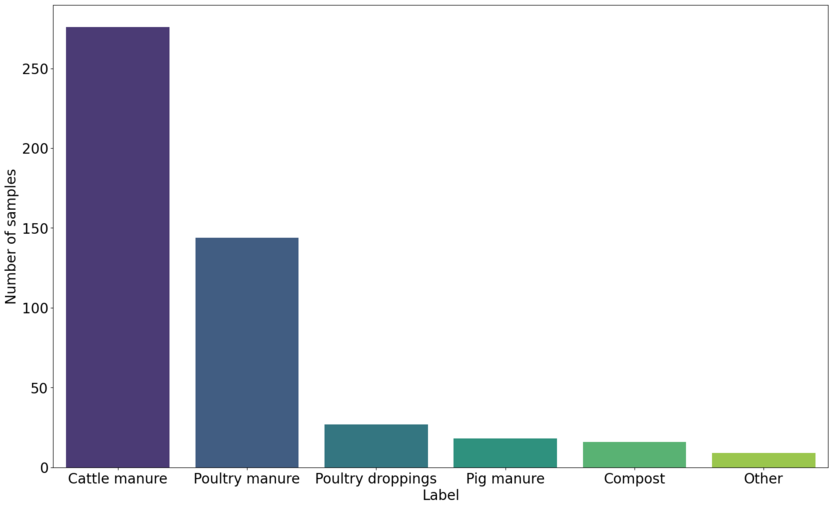
\includegraphics[width=\linewidth]{figs/Fig4.png}
        \caption{Number of Samples per Class in the Manure NIR dataset}
        \label{fig4}
    \end{subfigure}
    \hfill
    \begin{subfigure}[b]{0.48\textwidth}
        \centering
        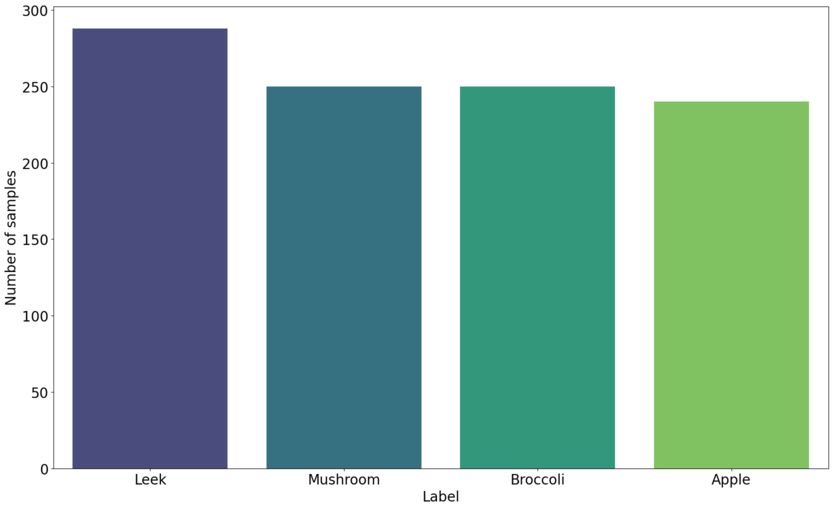
\includegraphics[width=\linewidth]{figs/Fig5.png}
        \caption{Number of Samples per Class in the Fruit NIR dataset}
        \label{fig5}
    \end{subfigure}
    \caption{Comparison of sample distributions between the Manure and Fruit NIR datasets}
    \label{fig4-5}
\end{figure}

\subsubsection{Image Dataset} For our image classification experiments, we utilize two publicly available datasets: the Danang Forest Plant Species dataset and the Macroscopic Image of Wood dataset.

The Danang Forest Plant Species, sourced from \cite{van2023plantkvit}, includes 489 plant species collected for project 36/HDKHCN/2020. Samples were manually gathered from four research areas in Da Nang, Vietnam, by expert botanists over a year as part of the project “Research on Building an Intelligent Management System of Flora in Da Nang.” The dataset comprises 487 species, encompassing a total of 10,576 images. Figure \ref{fig6} illustrates the distribution of samples per class in the Da Nang Forest Plant Species Dataset, revealing that most classes contain fewer than 20 images.

To construct a comprehensive Macroscopic Image of Wood dataset, four distinct datasets, Tropical Forest Species \cite{filho2014forest}, Brazilian Flora Species\cite{cano2022tropical}, Wood Species Dataset\cite{barmpoutis2018wood}, and Forest Species Database\cite{souza2020automatic}, were systematically integrated. This integration aimed to enhance taxonomic diversity, thereby improving classification performance. During data preparation, images belonging to classes with identical names were consolidated to ensure consistency. Furthermore, taxonomic nomenclature errors introduced during data collection were rigorously reviewed and rectified to align with standardized species names, facilitating the accurate aggregation of corresponding image collections. As a result, the final curated dataset comprises 16,346 images representing 75 distinct species.

Both datasets exhibit significant imbalance, as described in Figure \ref{fig6} and \ref{fig7}, necessitating the implementation of appropriate corrective methods.

\begin{figure}[!ht]
    \centering
    \begin{subfigure}[b]{0.48\textwidth}
        \centering
        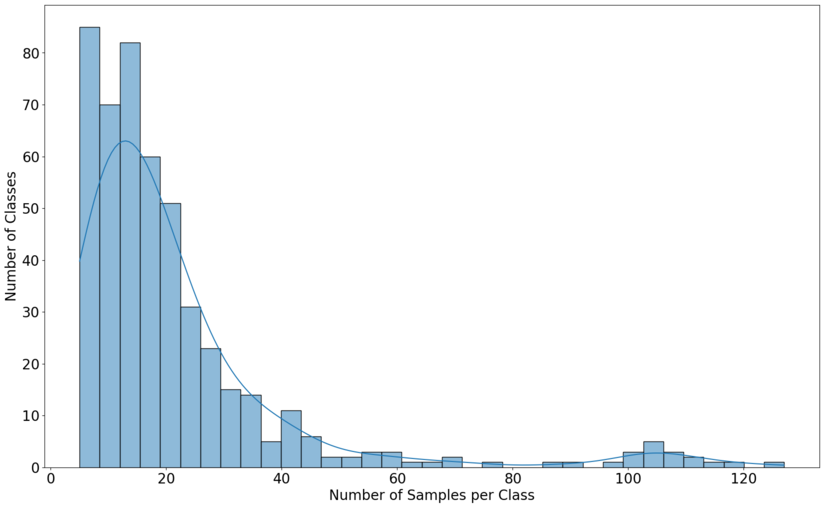
\includegraphics[width=\linewidth]{figs/Fig6.png}
        \caption{Distribution of Samples per Class in the Da Nang Forest Plant Species Dataset}
        \label{fig6}
    \end{subfigure}
    \hfill
    \begin{subfigure}[b]{0.48\textwidth}
        \centering
        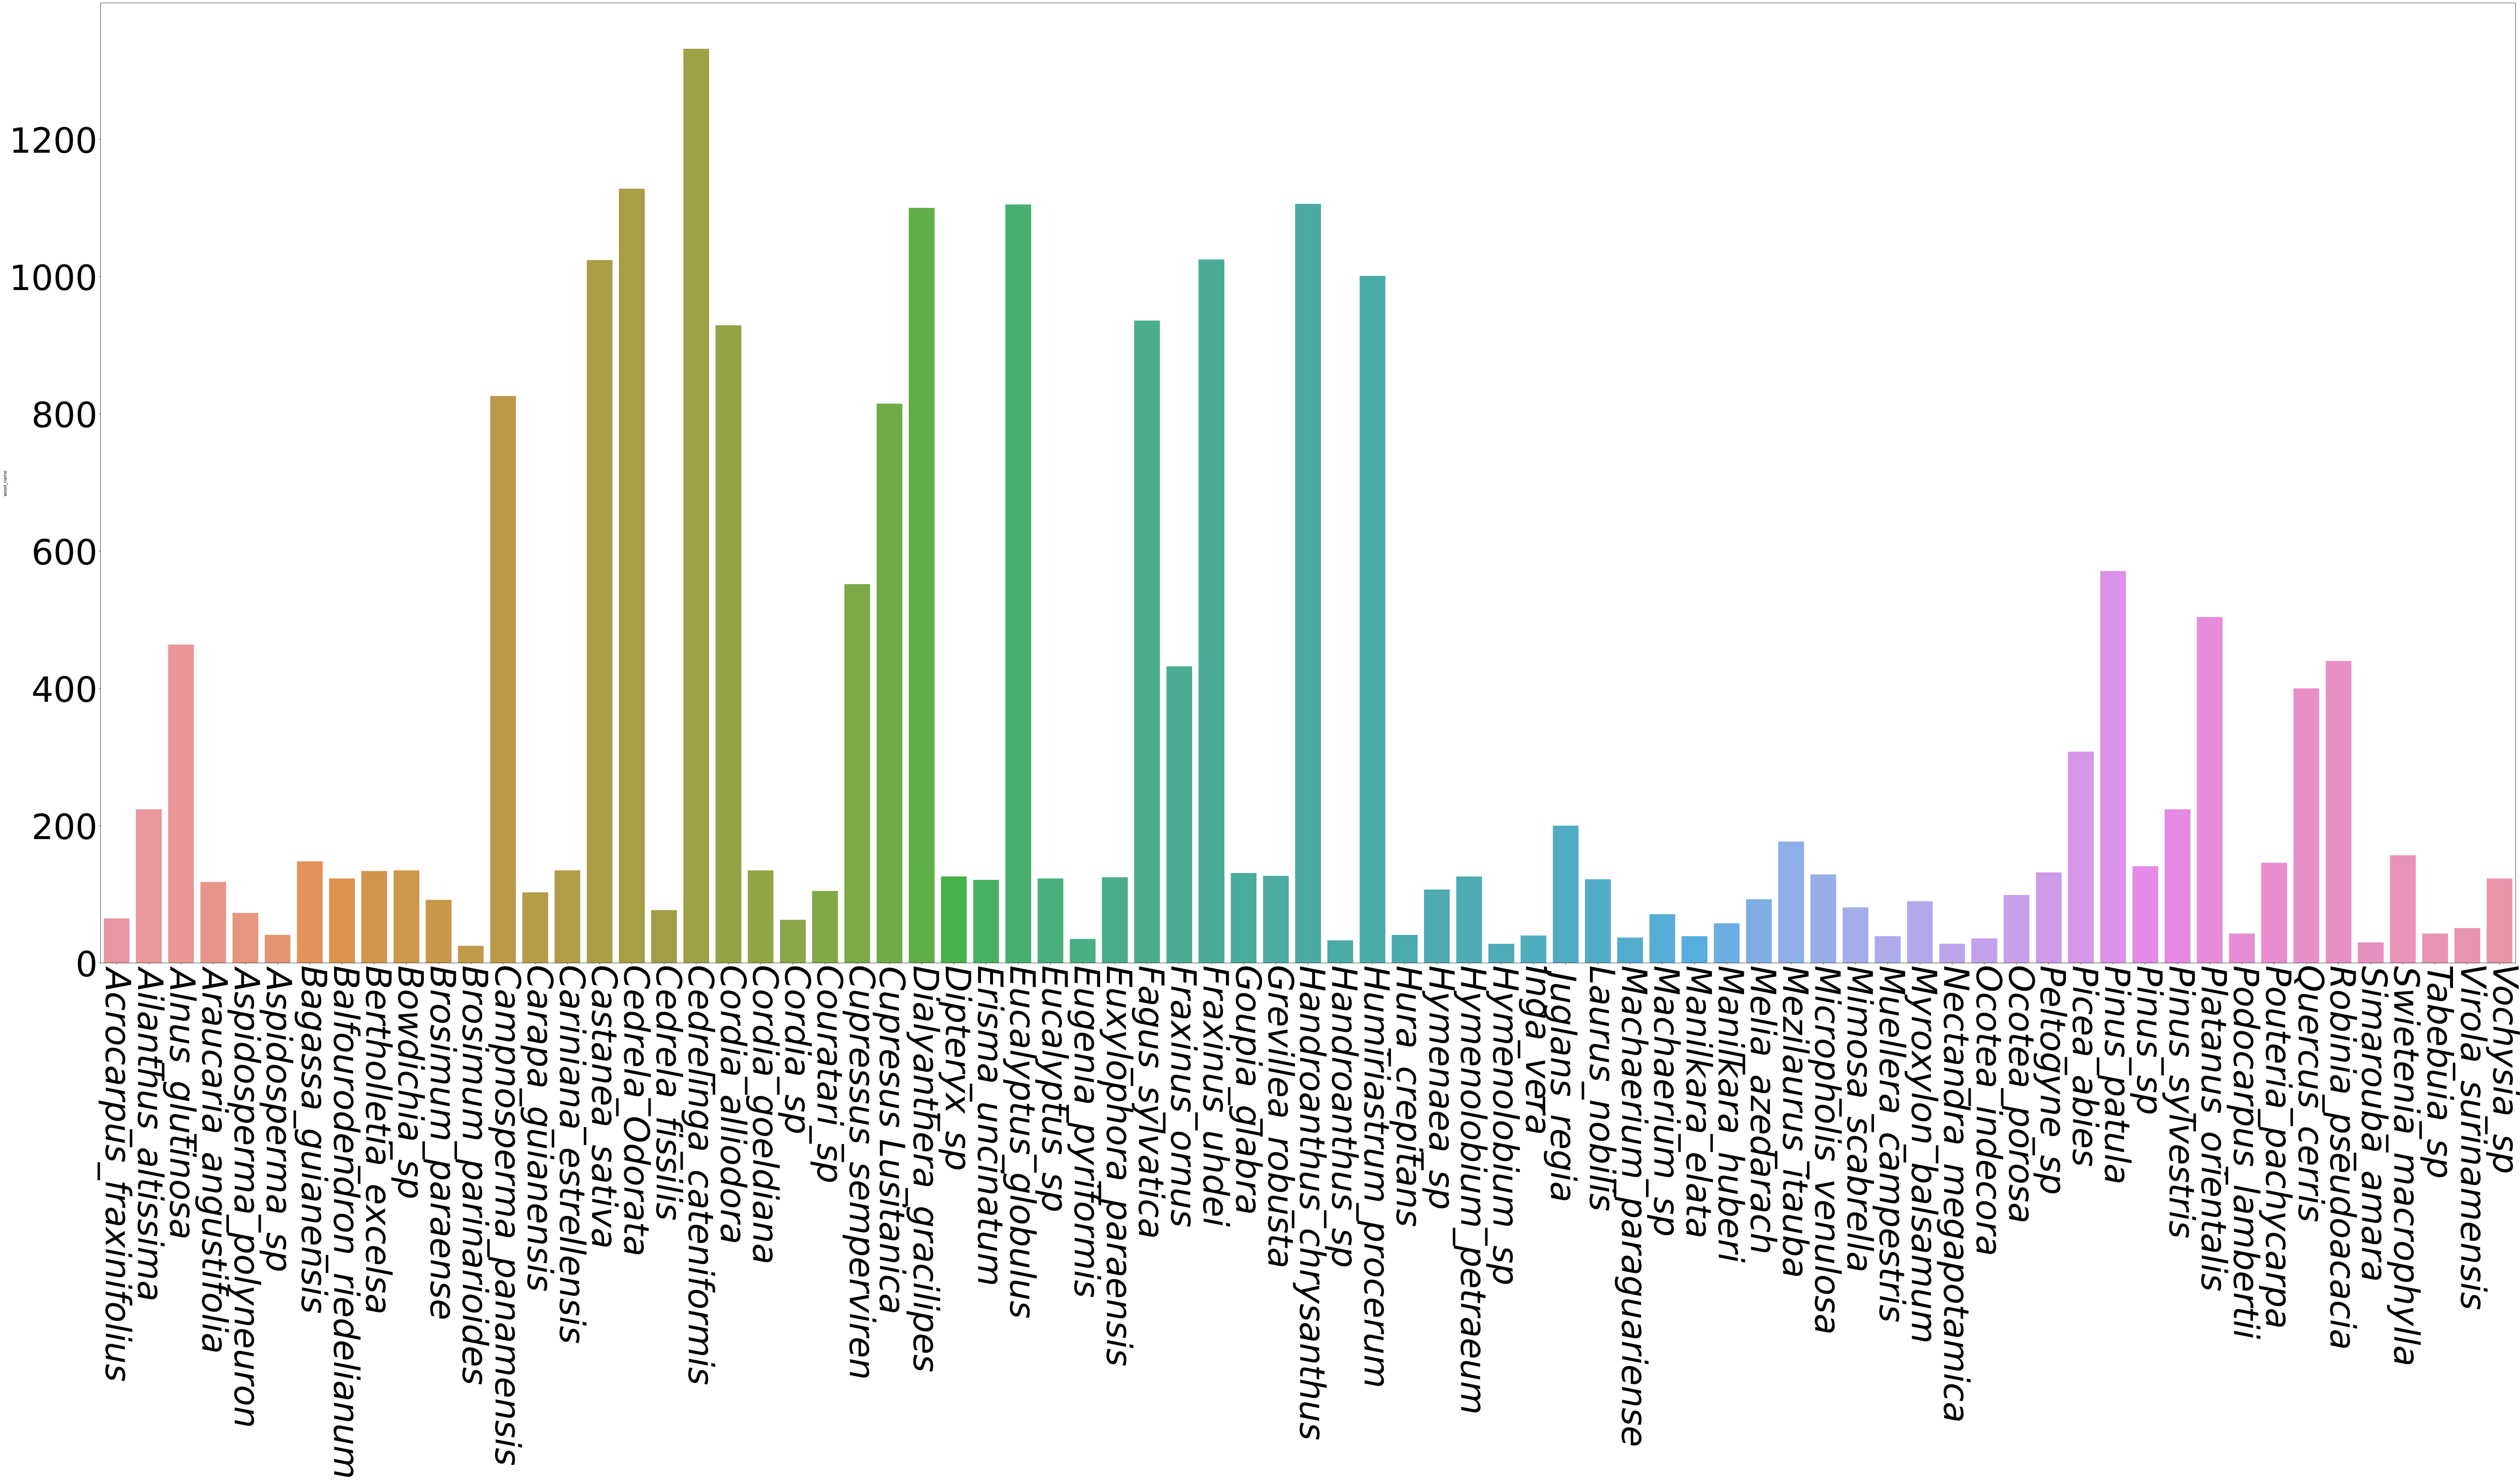
\includegraphics[width=\linewidth]{figs/Fig7.png}
        \caption{Number of Samples per Class in the Macroscopic Image of Wood dataset}
        \label{fig7}
    \end{subfigure}
    \caption{Comparison of sample distributions between the Da Nang Forest Plant Species and Macroscopic Image of Wood datasets}
    \label{fig6-7}
\end{figure}

\subsubsection{Text Dataset} 

The Massive Text Embedding Benchmark (MTEB) \cite{muennighoff2023mteb} provides a comprehensive evaluation framework for assessing text embedding models across multiple NLP tasks, including text classification covering 12 dataset. Built on the principles of diversity and broad applicability, MTEB is designed to evaluate the usability of embedding models across various real-world scenarios. The benchmark consists of eight distinct NLP tasks, each incorporating up to 15 datasets, amounting to a total of 58 datasets, of which 10 are multilingual, covering 112 different languages. For text classification, MTEB includes a diverse set of datasets spanning multiple domains and languages, enabling rigorous benchmarking of embedding-based models. By covering a wide range of classification tasks, ranging from binary sentiment analysis to multi-class topic categorization, MTEB facilitates a standardized comparison of embedding models’ generalization capabilities. Additionally, it incorporates both sentence-level and paragraph-level datasets, allowing for a comparative analysis of model performance on short and long text inputs.


\subsection{Preprocessing}
\subsubsection{Near-Infrared Spectroscopy Dataset} Following study \cite{hieu2024nirsvit}, to smooth spectral data, eliminate noise, and maintain continuity, the Savitzky-Golay filter is applied to every spectral range. This filter uses three polynomial orders with a window size of 21, making the data more suitable for deep learning model training. After the spectral data has been smoothed, the Standard Normal Variable (SNV) normalization method is applied. This technique brings the dataset to a mean of 0 and a standard deviation of 1, optimizing the processing workflow. The Upsampling method is employed as a corrective measure to address the data imbalance in the Manure NIR dataset.

\subsubsection{Image Dataset} 
Following the approach in \cite{van2023plantkvit}, image preprocessing is conducted before feeding the images into the model to enhance predictive performance. The preprocessing steps include:  
\begin{itemize}
    \item Cropping images at the center to improve feature extraction.
    \item Resizing images to a fixed dimension of \((224, 224)\).
    \item Normalizing pixel values using the parameters: \(mean = [0.485, 0.456, 0.406]\) and \(std = [0.229, 0.224, 0.225]\) for the three color channels.
    \item Applying data augmentation by generating additional images through random rotations within the range of -30 to 30 degrees and horizontal/vertical flipping.
\end{itemize}  
Additionally, to mitigate data imbalance, the Upsampling method is applied to the minority classes, increasing their sample size to approximate that of the majority class.

\subsubsection{Text Dataset} 
For text classification experiments, the tokenizers corresponding to each pretrained model from Hugging Face, as referenced in study \cite{muennighoff2023mteb}, are utilized to ensure model compatibility.

\subsection{Experiment Settings}
All experiments were conducted on an Ubuntu 20.04 system using the PyTorch 1.12.1 framework, Python 3.10.4, and an NVIDIA DGX A100 GPU with CUDA 12.1, powered by an Intel Xeon Platinum 8470Q CPU.

This study employs a diffusion model based on the original DDPM training strategy \cite{ho2020denoising}. To be more specific, each timestep \(t\) is sampled randomly and independently from the set of integers \(\{1, 2, ..., T\}\). Additionally, the noise level is scheduled following a linear process, with values set at \( \beta_1 = 1 \times 10^{-4} \) and \( \beta_T = 0.02 \).

The Data Encoder, Local Encoder, and Global Encoder modules employ distinct backbone architectures tailored to specific classification tasks. For NIR classification, all three encoders utilize the ResNet1D96 backbone, with configuration parameters defined in \cite{hong2020holmes}. In the case of image classification, ResNet101 \cite{he2016deep} is adopted as the shared backbone across all encoders. For text classification, a BERT-based \cite{devlin2019bert} model is consistently implemented across the three types of encoders.

Initially, the MCGM module and Data Encoder undergo a pre-training phase for 25 epochs, utilizing Cross Entropy as the loss function. Following this stage, the complete model, referred to as GuidedDCNet, is trained for 200 epochs, incorporating the pretrained weights from MCGM to enhance learning stability and convergence. Both training phases leverage the Adam optimization algorithm in conjunction with a cosine annealing scheduler. The initial learning rate is configured as \(5 \times 10^{-4}\) for the MCGM and Data Encoder, while the Unet model is assigned an initial learning rate of \(10^{-3}\). The hyperparameter \(\lambda\) in the total loss function \(\mathcal{L}_{total}\) is set to 0.5 in most experiments, as this value provides the best trade-off between guidance and reconstruction objectives. The detailed tuning and sensitivity analysis of \(\lambda\) are discussed in the Ablation Studies section.

To evaluate the performance of the model, k-fold cross-validation with \(k = 5\) was employed across the entire dataset. In this approach, the dataset is randomly partitioned into five equally sized folds. During each iteration, four folds are used for training, while the remaining fold is reserved for validation. This process is repeated five times, ensuring that each fold serves as the validation set exactly once. The final performance is calculated by averaging the results from all five iterations, providing a more reliable and robust estimate of the model's generalization capability. This method helps mitigate the effects of data variability and reduces the risk of overfitting, particularly when dealing with limited datasets.

\subsection{Experiment Results}
\subsubsection{Performance on NIR Classification}

The superior performance of GuidedDCNet on both NIR datasets demonstrates the effectiveness of its guided dual-consistency architecture. As shown in Table~\ref{tab1}, GuidedDCNet achieves the highest overall scores across all metrics, reaching 99.58\% accuracy on the Manure NIR dataset and 98.78\% accuracy on the Fruit NIR dataset, surpassing recent Transformer- and SSM-based methods such as NIRsViT and Mamba1D.

This improvement can be attributed to the specialized design of the Multi-Scale Cross-Guided Module (MSCGM) for spectral analysis. The global encoder captures the overall spectral distribution and mitigates baseline variations, while the local encoder, integrating SHAP-based interpretability and gated attention, focuses on characteristic absorption peaks essential for material discrimination. This dual-stream mechanism particularly benefits complex spectra such as Manure NIR, where overlapping peaks of C–H, O–H, and N–H bonds often challenge conventional models.

Moreover, the joint application of MMD regularization and the diffusion process further enhances robustness. The diffusion step suppresses spectral noise and corrects baseline shifts, while MMD regularization improves inter-class separability, enabling more reliable classification of spectrally similar samples. Overall, these synergistic components make GuidedDCNet a powerful and generalizable framework for NIR-based material recognition.

\begin{table}[!h]
\centering
\begin{threeparttable}
\caption{Quantitative results for NIR classification}
\label{tab1}
\renewcommand{\arraystretch}{1.0}
\begin{tabular}{ c c c c c c }
\hline
\textbf{Dataset} & \textbf{Method} & \textbf{\makecell{Accuracy \((\uparrow)\)}} & \textbf{\makecell{Precision \((\uparrow)\)}} & \textbf{\makecell{Recall \((\uparrow)\)}} & \textbf{\makecell{F1-Score \((\uparrow)\)}} \\ 
\hline
\multirow{5}{*}{\makecell{Manure \\ NIR}} 
& MLP \cite{popescu2009multilayer} & 95.96 & 91.43 & 86.73 & 89.01 \\
& ResNet1D96 \cite{hong2020holmes} & 97.67 & 96.26 & 85.42 & 90.51 \\
& NIRsViT \cite{hieu2024nirsvit} & 98.10 & 96.78 & 91.21 & 93.91 \\
& Mamba1D \cite{gu2024mamba} & 98.46 & 97.10 & 90.92 & 93.90 \\
& GuidedDCNet & \textbf{99.58} & \textbf{97.23} & \textbf{93.50} & \textbf{95.33} \\
\hline
\multirow{5}{*}{\makecell{Fruit \\ NIR}} 
& MLP \cite{popescu2009multilayer} & 79.08 & 64.59 & 65.93 & 65.26 \\
& ResNet1D96 \cite{hong2020holmes} & 90.87 & 82.27 & 82.12 & 82.12 \\
& NIRsViT \cite{hieu2024nirsvit} & 91.12 & 92.27 & 89.08 & 90.65 \\
& Mamba1D \cite{gu2024mamba} & 94.56 & 92.01 & 88.46 & 90.18 \\
& GuidedDCNet & \textbf{98.78} & \textbf{96.74} & \textbf{91.11} & \textbf{93.84} \\
\hline
\end{tabular}
\begin{tablenotes}
\footnotesize
\item The best values are in \textbf{bold}.
\end{tablenotes}
\end{threeparttable}
\end{table}

\subsubsection{Performance on Image Classification}

The quantitative results in Table \ref{tab2} highlight the consistent superiority of the proposed GuidedDCNet over recent Transformer-, Mamba-, and diffusion-based architectures. The model achieves the highest accuracy and F1-score across both the Danang Forest Plant Species and Macroscopic Wood datasets, outperforming even advanced frameworks such as RepCond Diffusion Transformer and Spatial-Mamba.

The architecture demonstrates strong effectiveness in handling multi-scale visual representations. In the plant species task, the MSCGM module’s global guidance vector effectively captures holistic morphological structures, while the SHAP-guided local mechanism enhances the identification of discriminative traits such as leaf venation and contour variations. This multi-scale attention proves crucial for the highly imbalanced Danang Forest dataset, where subtle inter-class variations dominate.

Similarly, for the macroscopic wood dataset, the model leverages both global textural cues and micro-level wood grain patterns, enabling accurate cross-species recognition. The performance gain (F1 = 94.93\%) compared to MambaML (93.59\%) and RepCond Diffusion Transformer (94.47\%) demonstrates that GuidedDCNet achieves a more balanced trade-off between accuracy and model complexity (72.3 M parameters) (\ref{tab4}), validating the efficiency of its guided dual-constraint design.

\begin{table}[!h]
\centering
\begin{threeparttable}
\caption{Quantitative results for Image Classification.}
\label{tab2}
\renewcommand{\arraystretch}{1.0}
\begin{tabular}{ c c c c c c }
\hline
\textbf{Dataset} & \textbf{Method} & \textbf{\makecell{Accuracy \\ \((\uparrow)\)}} & \textbf{\makecell{Precision \\ \((\uparrow)\)}} & \textbf{\makecell{Recall \\ \((\uparrow)\)}} & \textbf{\makecell{F1-Score \\ \((\uparrow)\)}} \\ 
\hline
\multirow{8}{*}{\makecell{Danang \\ Forest \\ Plant \\ Species}} 
& ResNet101 \cite{he2016deep} & 61.41 & 56.10 & 59.32 & 57.82 \\
& Vision Transformer \cite{dosovitskiy2021an} & 79.51 & 78.65 & 77.57 & 77.93 \\
& ConvNeXtV2 \cite{hieu2024nirsvit} & 84.52 & 85.37 & 82.74 & 84.76 \\
& PlantKViT \cite{van2023plantkvit} & 84.66 & 83.10 & 84.22 & 83.44 \\
& MambaML \cite{zhu2025mambaml} & 87.94 & 86.52 & 84.30 & 85.39 \\
& Spatial-Mamba \cite{xiao2025spatial} & 88.66 & 87.80 & 85.91 & 86.84 \\
& GuidedDCNet & \textbf{90.67} & \textbf{89.00} & \textbf{86.44} & \textbf{87.70} \\
\hline
\multirow{8}{*}{\makecell{Macroscopic \\ Image \\ of \\ Wood}} 
& ResNet101 \cite{he2016deep} & 90.78 & 89.72 & 90.16 & 89.94 \\
& Vision Transformer \cite{dosovitskiy2021an} & 91.57 & 90.75 & 91.92 & 91.33 \\
& ConvNeXtV2 \cite{hieu2024nirsvit} & 94.10 & 92.54 & 92.31 & 92.42 \\
& PlantKViT \cite{van2023plantkvit} & 93.80 & 91.90 & 92.05 & 91.97 \\
& MambaML \cite{zhu2025mambaml} & 95.12 & 93.78 & 93.42 & 93.59 \\
& Spatial-Mamba \cite{xiao2025spatial} & 95.60 & 94.12 & 93.90 & 94.01 \\
& GuidedDCNet & \textbf{96.51} & \textbf{95.09} & \textbf{94.78} & \textbf{94.93} \\
\hline
\end{tabular}
\begin{tablenotes}
\footnotesize
\item The best values are in \textbf{bold}.
\end{tablenotes}
\end{threeparttable}
\end{table}

\subsubsection{Performance on Text Classification}

Across 12 text classification datasets from the MTEB benchmark, GuidedDCNet demonstrates competitive accuracy compared to recent SOTA models (Table \ref{tab3}). While it does not achieve the highest scores on average, GuidedDCNet performs comparably to large-scale Transformer variants such as DeBERTaV3 and ModernBERT in several domain-focused datasets, including Banking77, MTOPDomain, MTOPIntent, MassiveScenario, ToxicConversations, and TweetSentiment.

The model’s strength lies in its multi-level semantic guidance mechanism (MSCGM), where global guidance captures contextual and structural cues, and local guidance focuses on phrase-level and entity-specific semantics. This hierarchical design enables GuidedDCNet to handle both domain-specific classification (e.g., Banking77, MTOPDomain) and multi-intent understanding (e.g., MassiveScenario, MTOPIntent) effectively. Furthermore, the integrated diffusion-based semantic refinement helps mitigate contextual noise and clarify ambiguous text expressions, contributing to competitive performance even with substantially fewer parameters than large generative models like ST5-XXL (Table \ref{tab4}).

For large-scale sentiment and review datasets such as AmazonPolarity, AmazonReviews, IMDB, and Emotion Classification, high-capacity models like ST5-XXL, ModernBERT, and DeBERTaV3 maintain an advantage due to extensive pretraining and larger model sizes. Nevertheless, GuidedDCNet achieves a favorable balance between accuracy, interpretability, and computational efficiency, highlighting its adaptability across a wide variety of text classification tasks.

\begin{table}[!h]
\centering
\begin{threeparttable}
\caption{Accuracy Score for Text Classification}
\label{tab3}
\renewcommand{\arraystretch}{2.0}
\begin{tabular}{ c c c c c c c }
\hline
\hline
\textbf{Dataset} &
\textbf{\makecell{BERT\\-based\\ \cite{devlin2019bert}}} &
\textbf{\makecell{MiniLM-L12\\-Multilingual\\ \cite{wang2020minilm}}} &
\textbf{\makecell{ST5-XXL\\ \cite{ni2022sentence}}} &
\textbf{\makecell{DeBERTaV3\\ \cite{huang2024deberta}}} &
\textbf{\makecell{ModernBERT\\ \cite{warner2025smarter}}} &
\textbf{GuidedDCNet} \\
\hline
\hline
\makecell{AmazonCounterfactual\\Classification} & 74.25 & 71.57 & 77.07 & 79.60 & \textbf{80.10} & 78.67 \\
\hline
\makecell{AmazonPolarity\\Classification} & 71.33 & 69.21 & 92.79 & 94.20 & \textbf{94.60} & 80.26 \\
\hline
\makecell{AmazonReviews\\Classification} & 33.56 & 35.11 & 48.93 & 50.60 & \textbf{51.10} & 38.31 \\
\hline
\makecell{Banking77\\Classification} & 63.41 & 79.77 & 82.31 & 84.60 & \textbf{85.00} & 85.36 \\
\hline
\makecell{Emotion\\Classification} & 35.28 & 42.37 & 48.57 & 50.90 & \textbf{51.40} & 46.21 \\
\hline
\makecell{Imdb\\Classification} & 65.35 & 60.46 & 90.23 & 92.10 & \textbf{92.70} & 75.38 \\
\hline
\makecell{MassiveIntent\\Classification} & 59.88 & 66.84 & 73.44 & 75.40 & \textbf{76.10} & 73.42 \\
\hline
\makecell{MassiveScenario\\Classification} & 64.28 & 71.51 & 74.82 & 76.40 & \textbf{77.00} & 77.32 \\
\hline
\makecell{MTOPDomain\\Classification} & 82.63 & 87.06 & 92.49 & 94.20 & \textbf{94.70} & 94.44 \\
\hline
\makecell{MTOPIntent\\Classification} & 68.14 & 65.52 & 68.33 & 72.90 & \textbf{73.40} & 73.30 \\
\hline
\makecell{ToxicConversations\\Classification} & 70.00 & 66.07 & 70.04 & 74.60 & \textbf{75.10} & 74.19 \\
\hline
\makecell{TweetSentiment\\ExtractionClassification} & 51.81 & 56.12 & 62.01 & 64.20 & \textbf{64.80} & 63.48 \\
\hline
\hline
\makecell{Average} & 61.66 & 64.30 & 73.42 & 77.06 & \textbf{77.68} & 71.70 \\
\hline
\hline
\end{tabular}
\begin{tablenotes}
\footnotesize
\item The best values are in \textbf{bold}.
\end{tablenotes}
\end{threeparttable}
\end{table}

GuidedDCNet's unified architecture demonstrates remarkable dimensional adaptability while maintaining its core structural integrity. The key innovation lies in how the same architectural components flexibly handle different data dimensionality - from one-dimensional spectral sequences, through two-dimensional spatial patterns, to high-dimensional semantic representations. The diffusion process seamlessly adapts its denoising operations to match each data type's inherent structure without requiring fundamental architectural modifications. This dimensional flexibility is achieved while preserving the model's computational efficiency, as evidenced by the consistent parameter efficiency across all data types compared to specialized architectures (26.5M for 1D, 72.3M for 2D, and 207M vs for text models). The model's ability to maintain state-of-the-art performance across such dimensionally diverse tasks, while preserving its architectural consistency, validates our approach to creating a truly unified, dimensionally-adaptive framework for multi-modal classification tasks.

\begin{table}[!h]
\centering
\begin{threeparttable}
\caption{Model Parameters Comparison.}
\label{tab4}
\renewcommand{\arraystretch}{1.2}
\begin{tabular}{c c c c c c}
\hline
\multicolumn{2}{c}{\textbf{NIR}} & \multicolumn{2}{c}{\textbf{Image}} & \multicolumn{2}{c}{\textbf{Text}} \\
\hline
\textbf{Model} & \textbf{Parameters} & \textbf{Model} & \textbf{Parameters} & \textbf{Model} & \textbf{Parameters} \\
\hline
ResNet1D96 & \textbf{16.6M} & ResNet101 & 42.8M & BERT-based & 110M \\
NIRsViT & 29.3M & Vision Transformer & 88.0M & MiniLM-L12 & 118M \\
Mamba1D & 24.7M & ConvNeXtV2 & 88.7M & DeBERTaV3-Large & 435M \\
GuidedDCNet & 26.5M & PlantKViT & 86.2M & ModernBERT-Base & 160M \\
& & MambaML & 95.4M & STS-XXL & 4860M \\
& & Spatial-Mamba & 97.1M & GuidedDCNet & 207M \\
& & \makecell{RepCond \\ Diffusion \\ Transformer} & 103.6M & & \\
& & GuidedDCNet & 72.3M & & \\
\hline
\end{tabular}
\begin{tablenotes}
\footnotesize
\item The best values are in \textbf{bold}.
\end{tablenotes}
\end{threeparttable}
\end{table}

\subsubsection{Ablation Studies}

To evaluate the effectiveness of each architectural component in GuidedDCNet, we conduct comprehensive ablation studies across three different data modalities, as in Table \ref{tab5}, \ref{tab6}, \ref{tab7}. Starting with only the global stream architecture, we progressively add the local stream, diffusion process, and MMD regularizer to analyze their individual contributions.

On the Manure NIR dataset, the base model with only the global stream achieves 97.67 accuracy. Adding the local stream improves performance to 98.18, demonstrating the importance of multi-scale feature extraction in spectral analysis. The introduction of the diffusion process further enhances accuracy to 98.89, showing its effectiveness in handling spectral noise. The complete model with MMD regularizer achieves optimal performance at 99.58.
For the Macroscopic Image of Wood dataset, we observe similar progressive improvements: from baseline accuracy of 90.78 with global stream only, to 93.57 with local stream addition, 95.37 with diffusion process, and finally 96.51 with full architecture. Each component's contribution is particularly evident in precision and recall metrics, indicating improved feature discrimination capabilities. 

\begin{table}[!ht]
\centering
\begin{threeparttable}
\caption{Ablation Study in GuidedDCNet on Manure NIR dataset}
\label{tab5}
\begin{tabular}{ c c c c c }
\hline
\textbf{Method} & \textbf{\makecell{Accuracy \\ \((\uparrow)\)}} & \textbf{\makecell{Precision \\ \((\uparrow)\)}} & \textbf{\makecell{Recall \\ \((\uparrow)\)}} & \textbf{\makecell{F1-Score \\ \((\uparrow)\)}} \\ 
\hline
\makecell{GuidedDCNet w/o Local Stream, Diffusion, MMD regularizer} & 97.67 & 96.26 & 85.42 & 90.51 \\
\hline
\makecell{GuidedDCNet w/o Diffusion, MMD regularizer} & 98.18 & 96.59 & 88.47 & 92.35 \\
\hline
\makecell{GuidedDCNet w/o MMD regularizer} & 98.89 & 97.01 & 91.03 & 93.92 \\
\hline
GuidedDCNet & \textbf{99.58} & \textbf{97.23} & \textbf{93.50} & \textbf{95.33} \\
\hline
\end{tabular}
\begin{tablenotes}
\footnotesize
\item The best values are in \textbf{bold}.
\end{tablenotes}
\end{threeparttable}
\end{table}

To further enhance the interpretability of our model, we visualize the learned guidance maps at both global and local scales (Fig.~\ref{fig8}). The sample is selected from the Danang Forest Plant Species dataset, containing diverse tropical vegetation with complex backgrounds. The Global Guidance highlights regions across the entire image that contribute to the overall prediction, while the Local Guidance focuses on the discriminative regions, particularly the flower petals, demonstrating the model’s ability to capture meaningful features at different spatial scales.

\begin{figure}
    \centering
    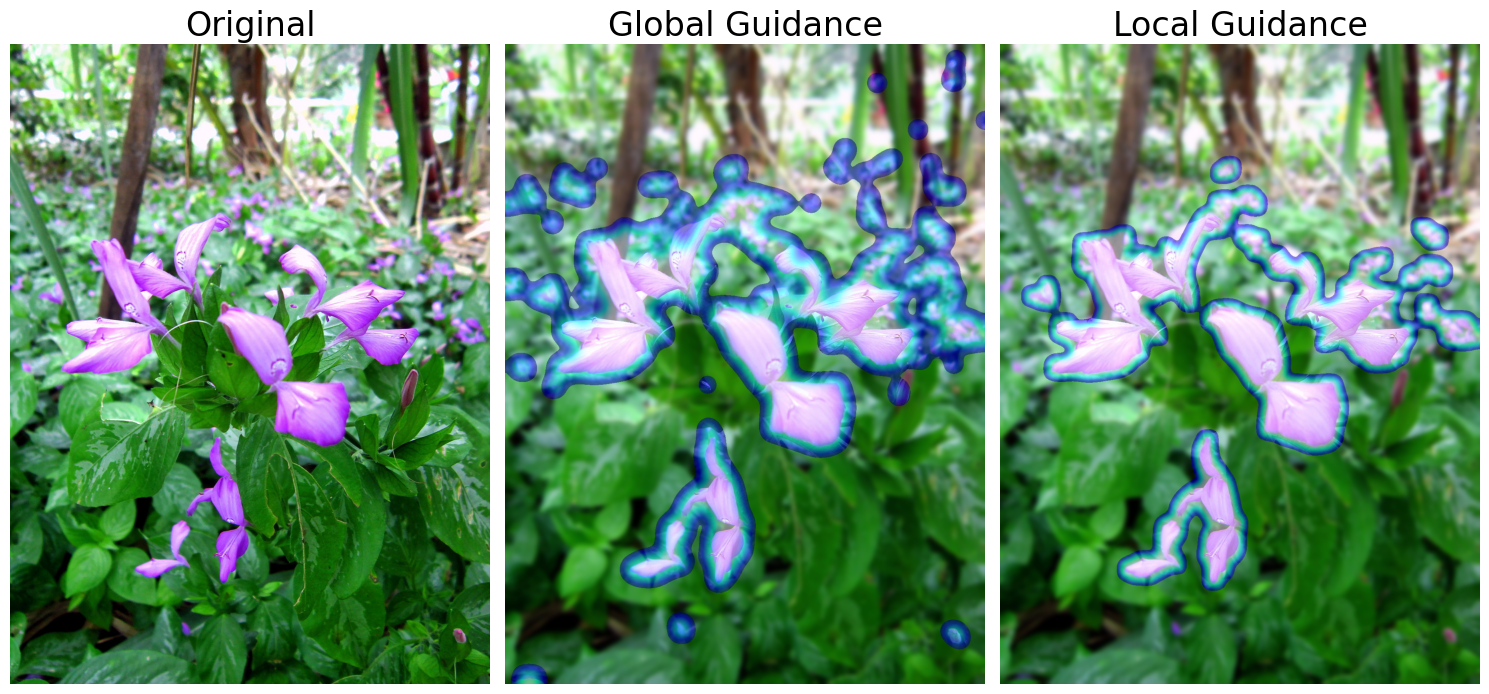
\includegraphics[width=0.8\linewidth]{figs/Fig8.png}
    \caption{Visualization of guidance vectors across multiple scales on a sample from the Da Nang Forest Plant Species dataset.}
    \label{fig8}
\end{figure}

\begin{table}[!ht]
\centering
\begin{threeparttable}
\caption{Ablation Study in GuidedDCNet on Macroscopic Image of Wood dataset}
\label{tab6}
\begin{tabular}{ c c c c c }
\hline
\textbf{Method} & \textbf{\makecell{Accuracy \\ \((\uparrow)\)}} & \textbf{\makecell{Precision \\ \((\uparrow)\)}} & \textbf{\makecell{Recall \\ \((\uparrow)\)}} & \textbf{\makecell{F1-Score \\ \((\uparrow)\)}} \\ 
\hline
\makecell{GuidedDCNet w/o Local Stream, Diffusion, MMD regularizer} & 90.78 & 89.72 & 90.16 & 89.94 \\
\hline
\makecell{GuidedDCNet w/o Diffusion, MMD regularizer} & 93.57 & 90.55 & 93.04 & 91.78 \\
\hline
\makecell{GuidedDCNet w/o MMD regularizer} & 95.37 & 94.26 & 93.15 & 93.70 \\
\hline
GuidedDCNet & \textbf{96.51} & \textbf{95.09} & \textbf{94.78} & \textbf{94.93} \\
\hline
\end{tabular}
\begin{tablenotes}
\footnotesize
\item The best values are in \textbf{bold}.
\end{tablenotes}
\end{threeparttable}
\end{table}

Text classification results on Amazon Reviews and Emotion Classification show consistent enhancement patterns. On Emotion Classification, accuracy improves from 35.28 to 38.12 with local stream addition, to 42.34 with diffusion, and reaches 46.21 with full architecture, demonstrating each component's role in handling semantic complexity.

These systematic improvements across all data modalities validate our architectural design choices and highlight how each component contributes meaningfully to the model's overall performance. The results demonstrate the complementary nature of our multi-scale feature extraction, diffusion-based denoising, and MMD regularization in achieving robust classification across diverse data types.

\begin{table}[!ht]
\centering
\begin{threeparttable}
\caption{Ablation Study on Text Dataset}
\label{tab7}
\begin{tabular}{ c c c c c c }
\hline
\textbf{Dataset} & \textbf{Method} & \textbf{\makecell{Accuracy \\ \((\uparrow)\)}} & \textbf{\makecell{Precision \\ \((\uparrow)\)}} & \textbf{\makecell{Recall \\ \((\uparrow)\)}} & \textbf{\makecell{F1-Score \\ \((\uparrow)\)}} \\ 
\hline
\multirow{4}{*}{\makecell{Amazon Reviews \\ Classification}} 
& \makecell{GuidedDCNet w/o Local Stream, \\ Diffusion, MMD regularizer} & 33.56 & 32.89 & 31.42 & 32.14 \\
\cline{2-6}
& \makecell{GuidedDCNet w/o Diffusion, \\ MMD regularizer} & 35.42 & 34.63 & 33.91 & 34.27 \\
\cline{2-6}
& \makecell{GuidedDCNet w/o \\ MMD regularizer} & 36.87 & 36.11 & 35.53 & 35.82 \\
\cline{2-6}
& GuidedDCNet & 38.31 & 37.52 & 37.04 & 37.28 \\
\hline
\multirow{4}{*}{\makecell{Emotion \\ Classification}} 
& \makecell{GuidedDCNet w/o Local Stream, \\ Diffusion, MMD regularizer} & 35.28 & 34.61 & 33.52 & 34.06 \\
\cline{2-6}
& \makecell{GuidedDCNet w/o Diffusion, \\ MMD regularizer} & 38.12 & 37.41 & 36.62 & 37.01 \\
\cline{2-6}
& \makecell{GuidedDCNet w/o \\ MMD regularizer} & 42.34 & 41.62 & 40.91 & 41.26 \\
\cline{2-6}
& GuidedDCNet & \textbf{46.21} & \textbf{45.51} & \textbf{45.02} & \textbf{45.26} \\
\hline
\end{tabular}
\begin{tablenotes}
\footnotesize
\item The best values are in \textbf{bold}.
\end{tablenotes}
\end{threeparttable}
\end{table}

To further analyze the interpretability and effectiveness of the proposed dual-guidance mechanism, we visualize the Global Guidance and Local Guidance matrices, as illustrated in Figure \ref{fig9}. The Global Guidance heatmap exhibits a distributed attention pattern, indicating that the model captures broad contextual dependencies among tokens (e.g., correlations between Good, value, and money). This demonstrates its capability to encode global semantic relations that contribute to the overall understanding of the input. In contrast, the Local Guidance heatmap shows highly concentrated activations on specific token groups (e.g., around Not, but, and does), reflecting the model’s ability to focus on fine-grained contextual cues and local consistency. These complementary behaviors confirm that the dual-guidance design enables the model to effectively learn multi-scale feature interactions, where global guidance provides semantic context while local guidance refines the representation with detail-oriented information.

\begin{figure}
    \centering
    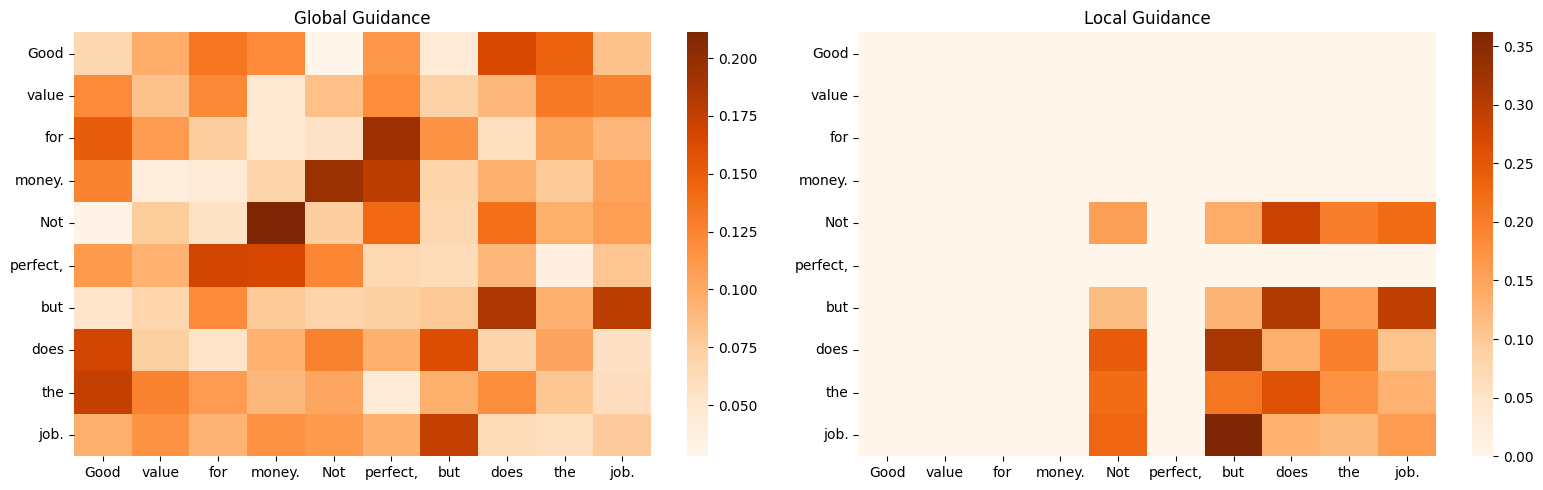
\includegraphics[width=\linewidth]{figs/Fig9.png}
    \caption{Visualization of guidance vectors across multiple scales on a sample from the Amazon Reviews Classification dataset.}
    \label{fig9}
\end{figure}

Tables~\ref{tab8} and~\ref{tab9} illustrate the influence of the trade-off parameter $\lambda$ on the performance of GuidedDCNet across different data modalities. For 1D and 2D datasets, the model maintains consistently high accuracy and F1-scores throughout the range $\lambda \in [0.3,0.7]$, with moderate values ($\lambda \approx 0.5 - 0.6$) yielding marginally superior outcomes. In the case of textual datasets, optimal performance is observed at $\lambda = 0.5$, whereas further increases in $\lambda$ result in a gradual decline in all metrics, suggesting that overly strong MMD regularization may attenuate essential semantic information. Collectively, these findings indicate that employing a moderate $\lambda$ achieves an effective balance between enforcing distributional alignment and preserving task-relevant feature representations.

\begin{table*}[htbp]
\centering
\caption{Performance of GuidedDCNet on Manure NIR and Macroscopic Image of Wood datasets with different $\lambda$ values.}
\label{tab8}
\begin{tabular}{c|cccc|cccc}
\hline
\multirow{2}{*}{$\lambda$} 
& \multicolumn{4}{c|}{\textbf{Manure NIR}} 
& \multicolumn{4}{c}{\textbf{Macroscopic Image of Wood}} \\ 
\cline{2-9}
& \makecell{Accuracy \\ \((\uparrow)\)} & \makecell{Precision \\ \((\uparrow)\)} & \makecell{Recall \\ \((\uparrow)\)} & \makecell{F1-Score \\ \((\uparrow)\)}
& \makecell{Accuracy \\ \((\uparrow)\)} & \makecell{Precision \\ \((\uparrow)\)} & \makecell{Recall \\ \((\uparrow)\)} & \makecell{F1-Score \\ \((\uparrow)\)} \\ 
\hline
0.3 & 99.56 & 97.15 & 93.40 & 95.30 
    & 96.40 & 94.95 & 94.60 & 94.77 \\
0.4 & 99.60 & 97.20 & 93.48 & 95.38 
    & 96.48 & 95.03 & 94.72 & 94.88 \\
0.5 & \textbf{99.58} & \textbf{97.23} & \textbf{93.50} & \textbf{95.33} 
    & \textbf{96.51} & \textbf{95.09} & \textbf{94.78} & \textbf{94.93} \\
0.6 & 99.62 & 97.30 & 93.55 & 95.42 
    & 96.55 & 95.15 & 94.80 & 94.98 \\
0.7 & 99.55 & 97.10 & 93.30 & 95.17 
    & 96.45 & 95.05 & 94.60 & 94.82 \\
\hline
\end{tabular}
\end{table*}

\begin{table*}[htbp]
\centering
\caption{Performance of GuidedDCNet on textual data with $\lambda$ values}
\label{tab9}
\begin{tabular}{c|cccc|cccc}
\hline
\multirow{2}{*}{$\lambda$} 
& \multicolumn{4}{c|}{\textbf{Amazon Reviews}} 
& \multicolumn{4}{c}{\textbf{Emotion}} \\ 
\cline{2-9}
& \makecell{Accuracy \\ \((\uparrow)\)} & \makecell{Precision \\ \((\uparrow)\)} & \makecell{Recall \\ \((\uparrow)\)} & \makecell{F1-Score \\ \((\uparrow)\)}
& \makecell{Accuracy \\ \((\uparrow)\)} & \makecell{Precision \\ \((\uparrow)\)} & \makecell{Recall \\ \((\uparrow)\)} & \makecell{F1-Score \\ \((\uparrow)\)} \\ 
\hline
0.3 & 38.70 & 38.00 & 37.60 & 37.80 
    & 46.50 & 45.85 & 45.45 & 45.65 \\
0.4 & 38.45 & 37.75 & 37.40 & 37.57 
    & 46.30 & 45.70 & 45.25 & 45.47 \\
0.5 & \textbf{38.31} & \textbf{37.52} & \textbf{37.04} & \textbf{37.28} 
    & \textbf{46.21} & \textbf{45.51} & \textbf{45.02} & \textbf{45.26} \\
0.6 & 37.90 & 37.10 & 36.70 & 36.90 
    & 45.90 & 45.20 & 44.80 & 45.00 \\
0.7 & 37.20 & 36.50 & 36.10 & 36.30 
    & 45.40 & 44.75 & 44.30 & 44.52 \\
\hline
\end{tabular}
\end{table*}

In recent studies, various works have compared SHAP- and GradCAM-based interpretability mechanisms to better understand their trade-offs across different domains. For instance, Van et al. \cite{van2024harnessing} demonstrated that while SHAP provides fine-grained feature attribution suitable for non-visual or heterogeneous data, Grad-CAM excels in generating spatially coherent saliency maps for visual tasks. Similarly, comparative analyses on image explanation similarity \cite{yavtukhovskyi2025evaluation} have revealed that SHAP and Grad-CAM often produce complementary rather than identical interpretations, each emphasizing different aspects of model behavior.

In the context of this study, the MSCGM mechanism adopts SHAP-based local feature extraction because it is model-agnostic and capable of quantifying feature importance across diverse data modalities, including non-visual representations such as spectroscopy and text. Grad-CAM, while efficient in visual domains, is inherently gradient-dependent and spatially constrained, making it less suitable for the generalized, modality-independent framework proposed in GuidedDCNet. Nevertheless, exploring lightweight gradient-based interpretability methods remains an interesting future direction, particularly for extending MSCGM to visual or hybrid multimodal applications.

\section{Conclusion}

This paper presents GuidedDCNet, a novel diffusion-integrated framework that advances the state-of-the-art in data classification across multiple modalities. The key innovation lies in the integration of two complementary components: a Multi-scale Conditional Guidance Mechanism that effectively combines global and local feature analysis, and a diffusion process that systematically reduces noise while preserving discriminative features.

Our comprehensive evaluation demonstrates GuidedDCNet's effectiveness and architectural consistency across three distinct data types. For NIR spectroscopy classification, the model achieves superior accuracies of 99.58\% (Manure) and 98.78\% (Fruit) with only 26.5M parameters, surpassing previous methods like NIRsViT and ResNet1D96. Similarly, for image datasets, it maintains high performance with 90.67\% (Danang Forest Plants) and 96.51\% (Wood) accuracy using 72.3M parameters, outperforming established architectures like ConvNeXtV2  and Vision Transformer. In text classification across the MTEB benchmark, despite using only 207M parameters compared to ST5-XXL's 4860M, our model achieves a competitive performance of 71.70\% average accuracy (versus 73.42\%) and excels in 7 out of 12 specific tasks, notably surpassing BERT-based (61.66\%) and MiniLM-L12 (64.30\%) models. These results demonstrate consistent high performance across diverse data modalities while maintaining significant parameter efficiency compared to specialized architectures.

The ablation studies validate the contribution of each architectural component, with the combination of MSCGM, diffusion process, and MMD regularization collectively enhancing classification performance. Additionally, GuidedDCNet maintains parameter efficiency across data modalities (26.5M for 1D, 72.3M for 2D, and 207M for text) while achieving competitive or superior results compared to specialized architectures.

Future research will focus on extending GuidedDCNet to lightweight and streaming scenarios for real-time applications, and exploring hybrid interpretability strategies that integrate gradient-based methods with SHAP-inspired mechanisms to improve scalability and efficiency. In addition, incorporating self-supervised pretraining and cross-modal knowledge transfer represents a promising direction to further enhance the model’s adaptability across diverse multimodal tasks.

\section{Acknowledgements} This work was funded by The University of Danang, University of Science and Technology.

% To print the credit authorship contribution details
\printcredits

%% Loading bibliography style file
\bibliographystyle{cas-model2-names}

% Loading bibliography database
\bibliography{cas-refs}

\end{document}

